%!TEX root = ../dissertation.tex
\begin{savequote}[75mm]
The treasure in my mind is greater than any worldly glory.   
\end{savequote}
\chapter{Constant \muqcd~ Validation}
\label{AppendixMuqcd}

\paragraph{}
One important assumption of this analysis is the constancy \muqcd~ across different regions on the 2D \mleadJ-\msublJ~ plane. 
This can be validated in data, excluding signal regions, which were blinded during this check. 
The \ttbar~ contribution is estimated directly from MC and subtracted in the data distributions. 
The ratio of the number of n-$b$-tagged events versus the number of less-$b$-tagged events in each \mleadJ-\msublJ bin is calculated.
The pull of the ratios in SB/CR/SR is also calculated.
These two distributions shows the consistency of \muqcd~ in SB/CR/SR, as seen in Figures~\ref{fig:app-muqcd-1b} ($1b$ over $0b$), ~\ref{fig:app-muqcd-2b} ($2b$ over $1b$), ~\ref{fig:app-muqcd-2bs} ($2bs$ over $1b$), ~\ref{fig:app-muqcd-3b} ($3b$ over $2b$), ~\ref{fig:app-muqcd-4b} ($4b$ over $2b$). 
Table~\ref{tab:bkgfit} compares the \muqcd~ value in the $4b/3b/2bs$ channels.
This validates the choice of sideband region and the assumption of \muqcd~ as constant in the analysis.


\begin{figure}[htb!]
\centering
\captionsetup{justification=centering}
	\hspace{-1cm}
    \begin{subfigure}[b]{0.4\textwidth}
        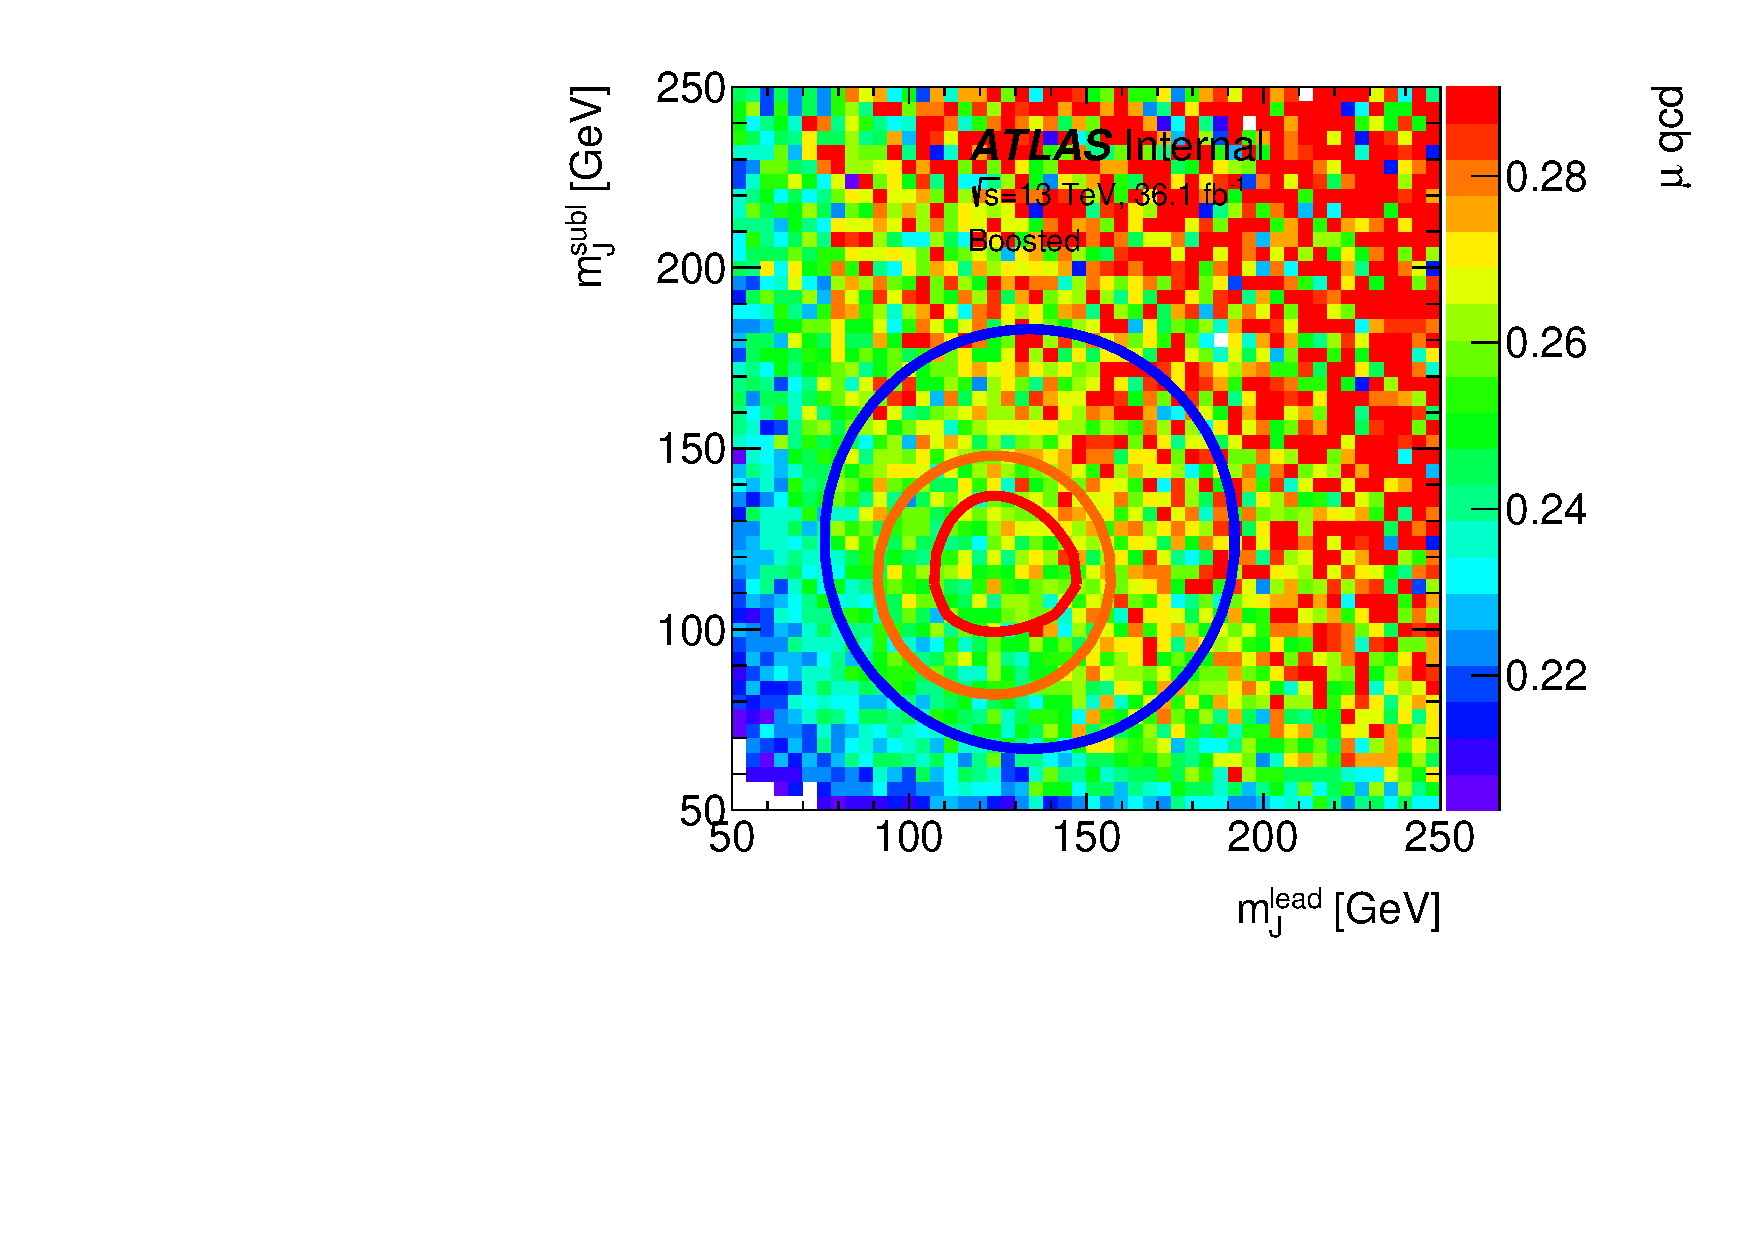
\includegraphics[width=\textwidth,angle=-90]{figures/boosted/AppendixMuqcdstudy/OneTag_Incl_mH0H1.pdf}
        \caption{\muqcd~ on the \mleadJ-\msublJ~ plane}
        \label{fig:app-muqcd-1b-2d}
    \end{subfigure}
    \quad \quad \quad \quad 
    \begin{subfigure}[b]{0.4\textwidth}
        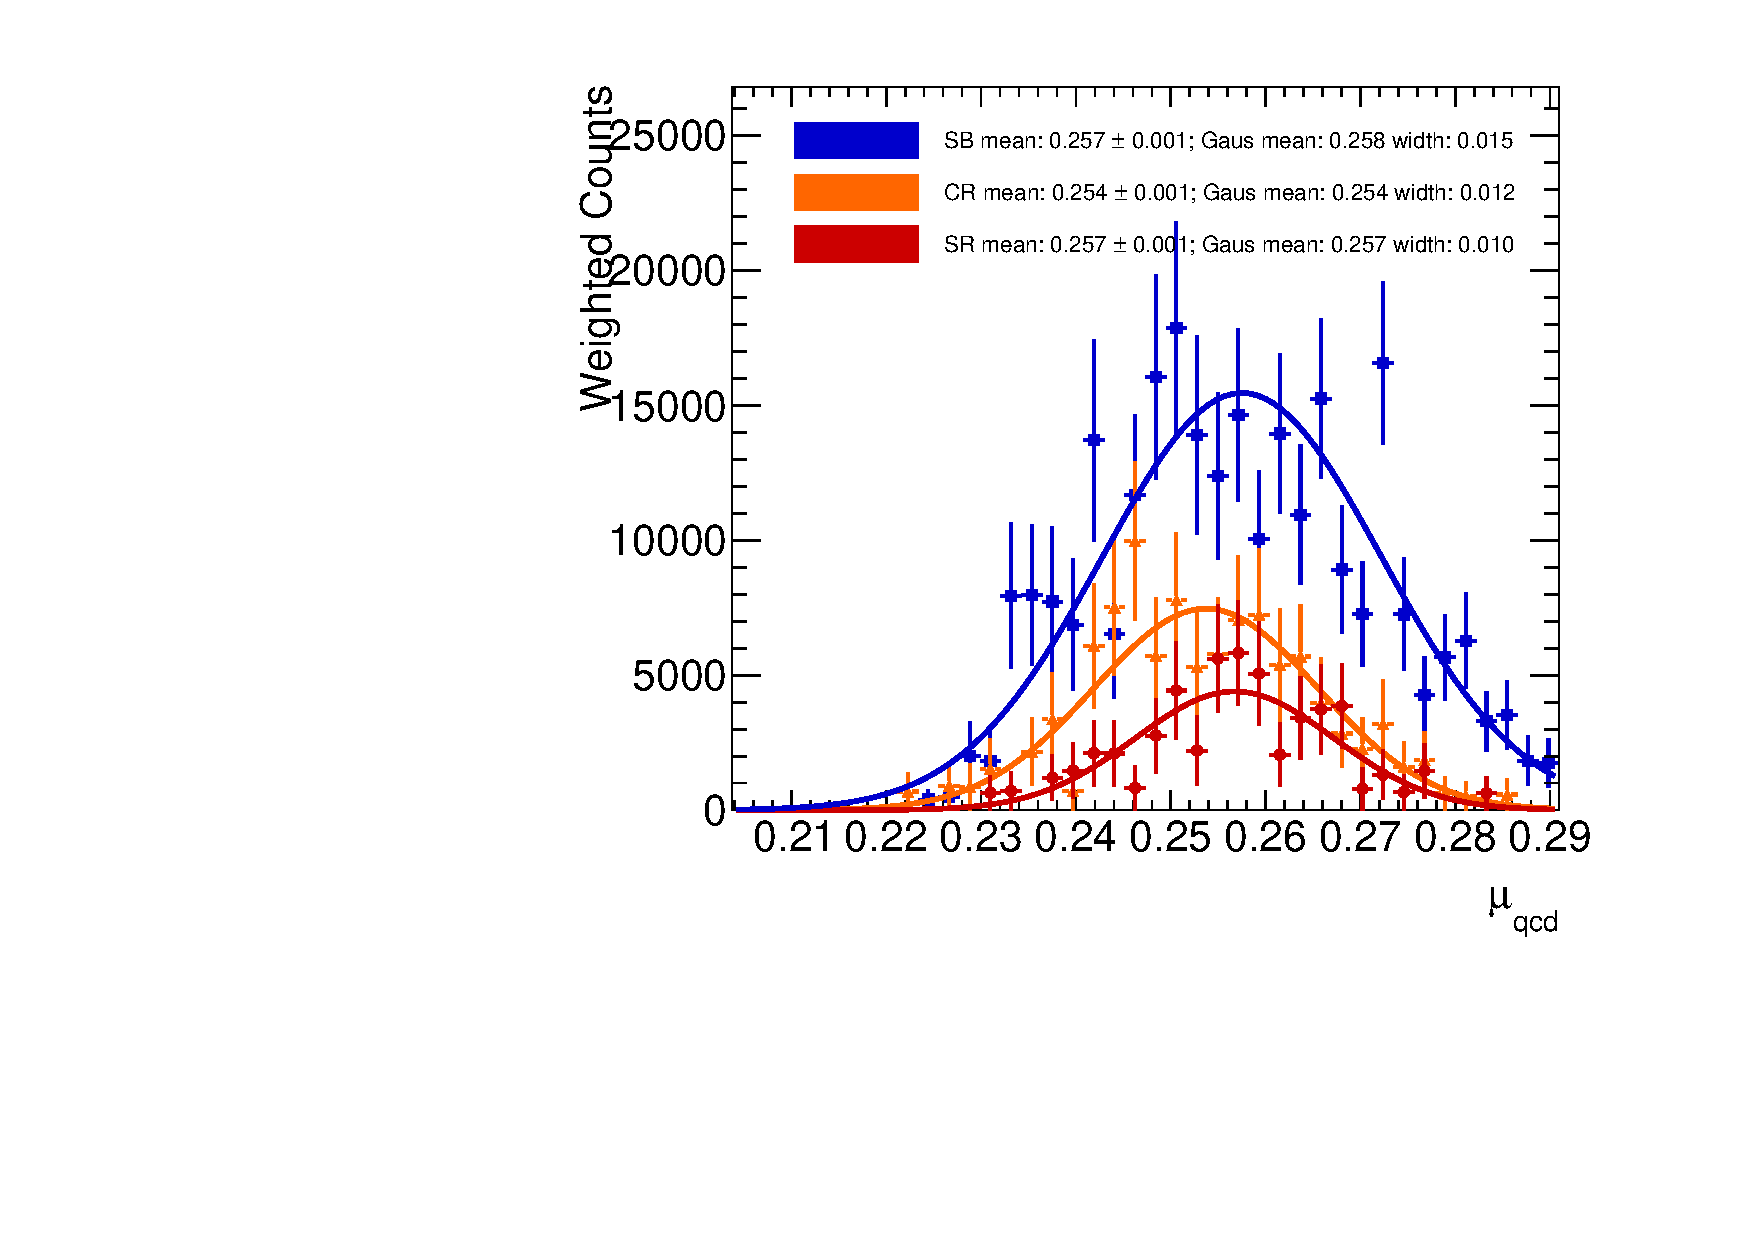
\includegraphics[width=\textwidth,angle=-90]{figures/boosted/AppendixMuqcdstudy/OneTag_Incl_mH0H1_pull.pdf}
        \caption{pulled \muqcd~ distribution in SB/CR/SR}
        \label{fig:app-muqcd-1b-pull}
    \end{subfigure}
\caption{$1b$ over $0b$ \muqcd~ values evaluated in data, with the $N_{event}$ weighted mean and the Gaussian fit mean listed.}
\label{fig:app-muqcd-1b}
\end{figure}

\begin{figure}[htb!]
\centering
\captionsetup{justification=centering}
	\hspace{-1cm}
    \begin{subfigure}[b]{0.4\textwidth}
        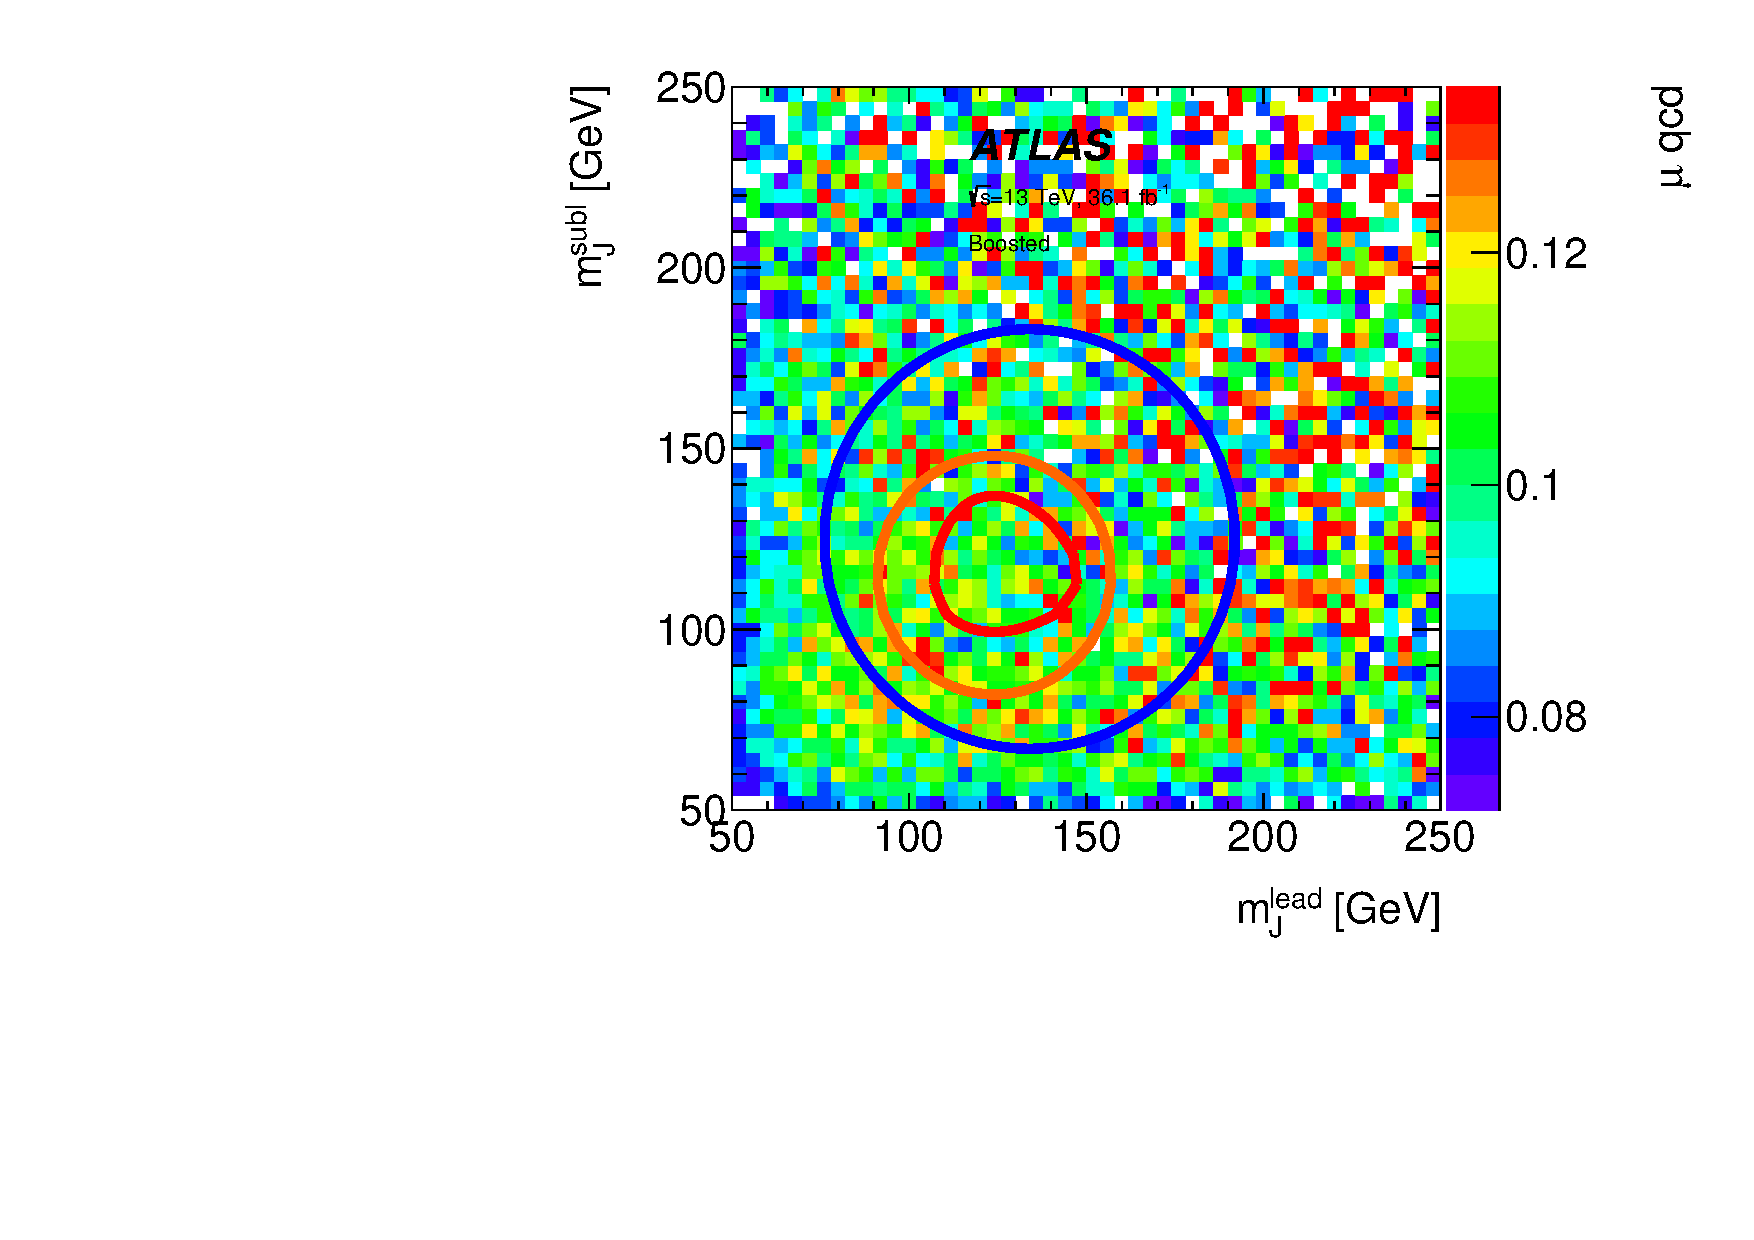
\includegraphics[width=\textwidth,angle=-90]{figures/boosted/AppendixMuqcdstudy/TwoTag_Incl_mH0H1.pdf}
        \caption{\muqcd~ on the \mleadJ-\msublJ~ plane}
        \label{fig:app-muqcd-2b-2d}
    \end{subfigure}
    \quad \quad \quad \quad 
    \begin{subfigure}[b]{0.4\textwidth}
        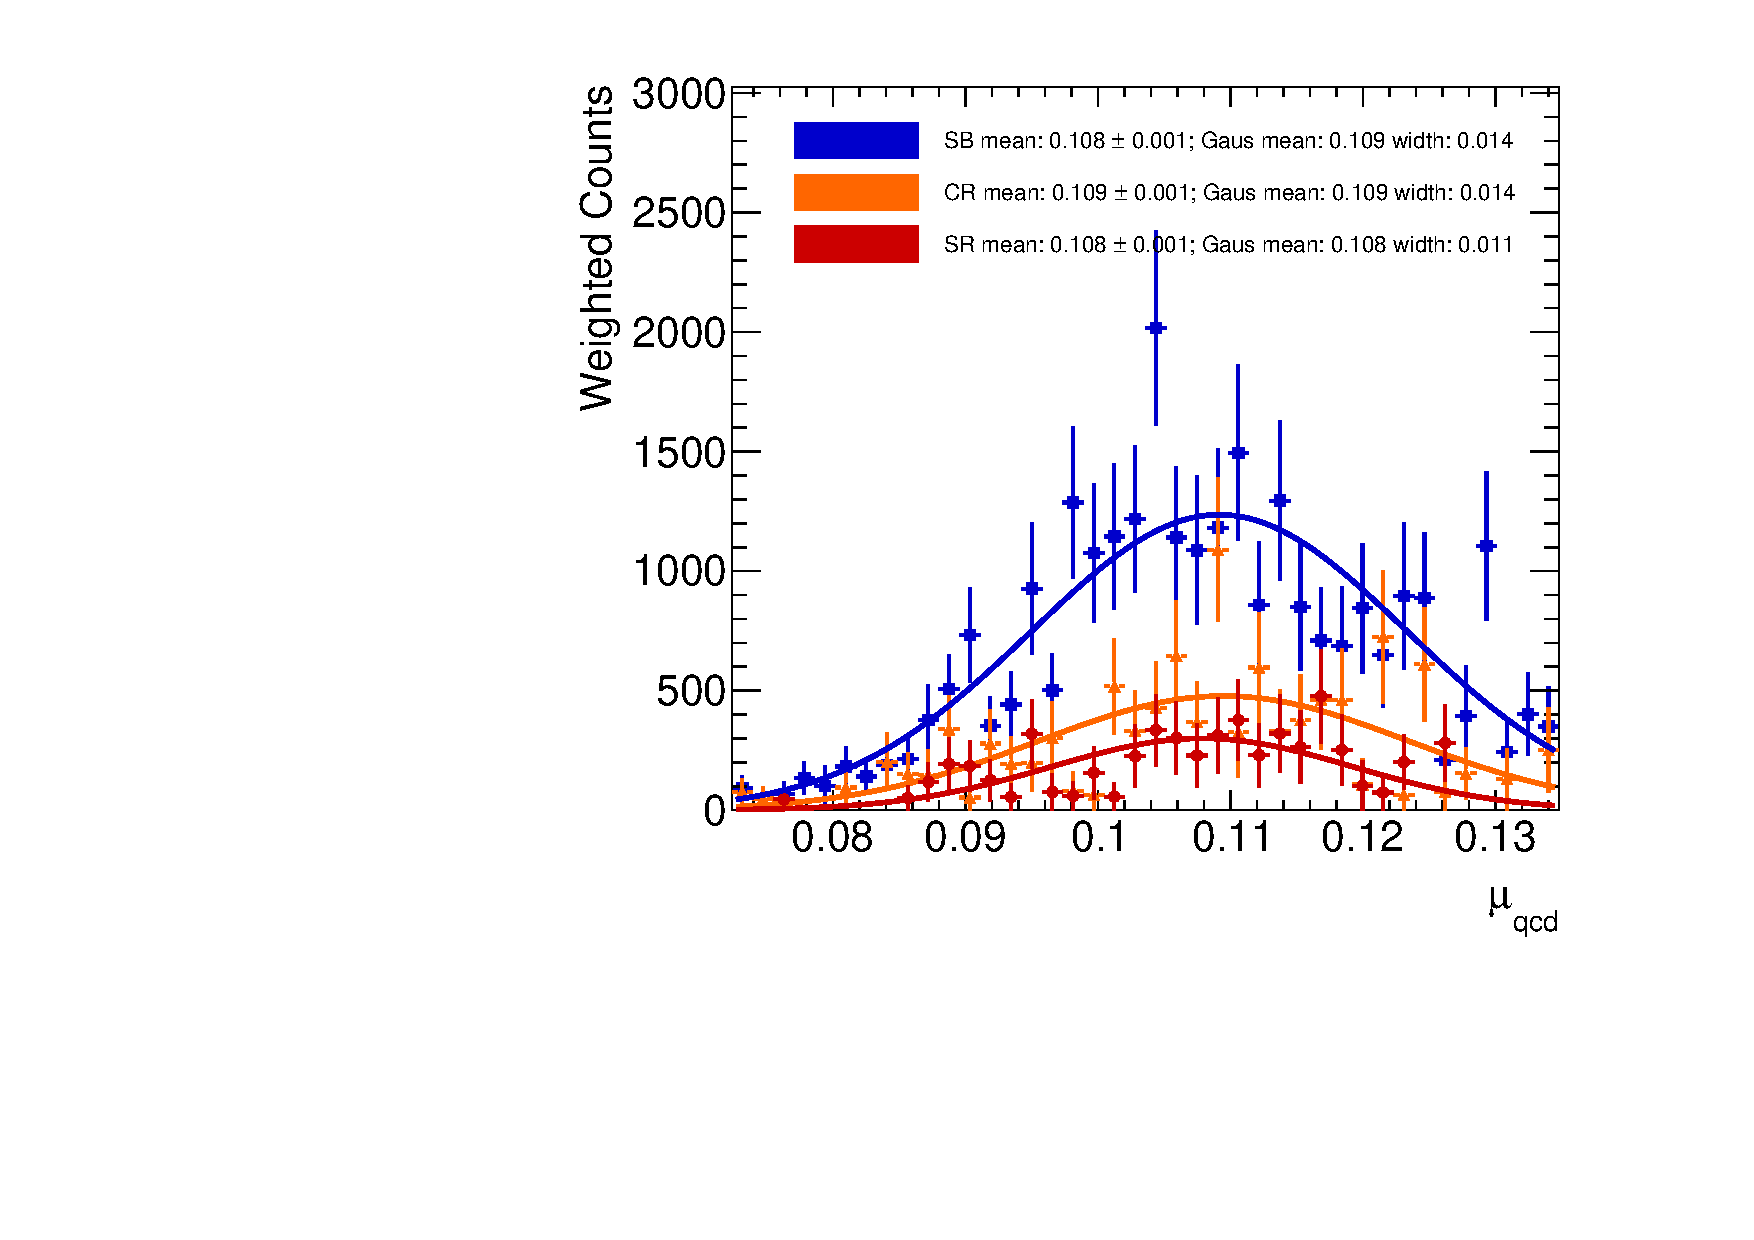
\includegraphics[width=\textwidth,angle=-90]{figures/boosted/AppendixMuqcdstudy/TwoTag_Incl_mH0H1_pull.pdf}
        \caption{pulled \muqcd~ distribution in SB/CR/SR}
        \label{fig:app-muqcd-2b-pull}
    \end{subfigure}
\caption{$2b$ over $1b$ \muqcd~ values evaluated in data, with the $N_{event}$ weighted mean and the Gaussian fit mean listed.}
\label{fig:app-muqcd-2b}
\end{figure}

\begin{figure}[htb!]
\centering
\captionsetup{justification=centering}
	\hspace{-1cm}
    \begin{subfigure}[b]{0.4\textwidth}
        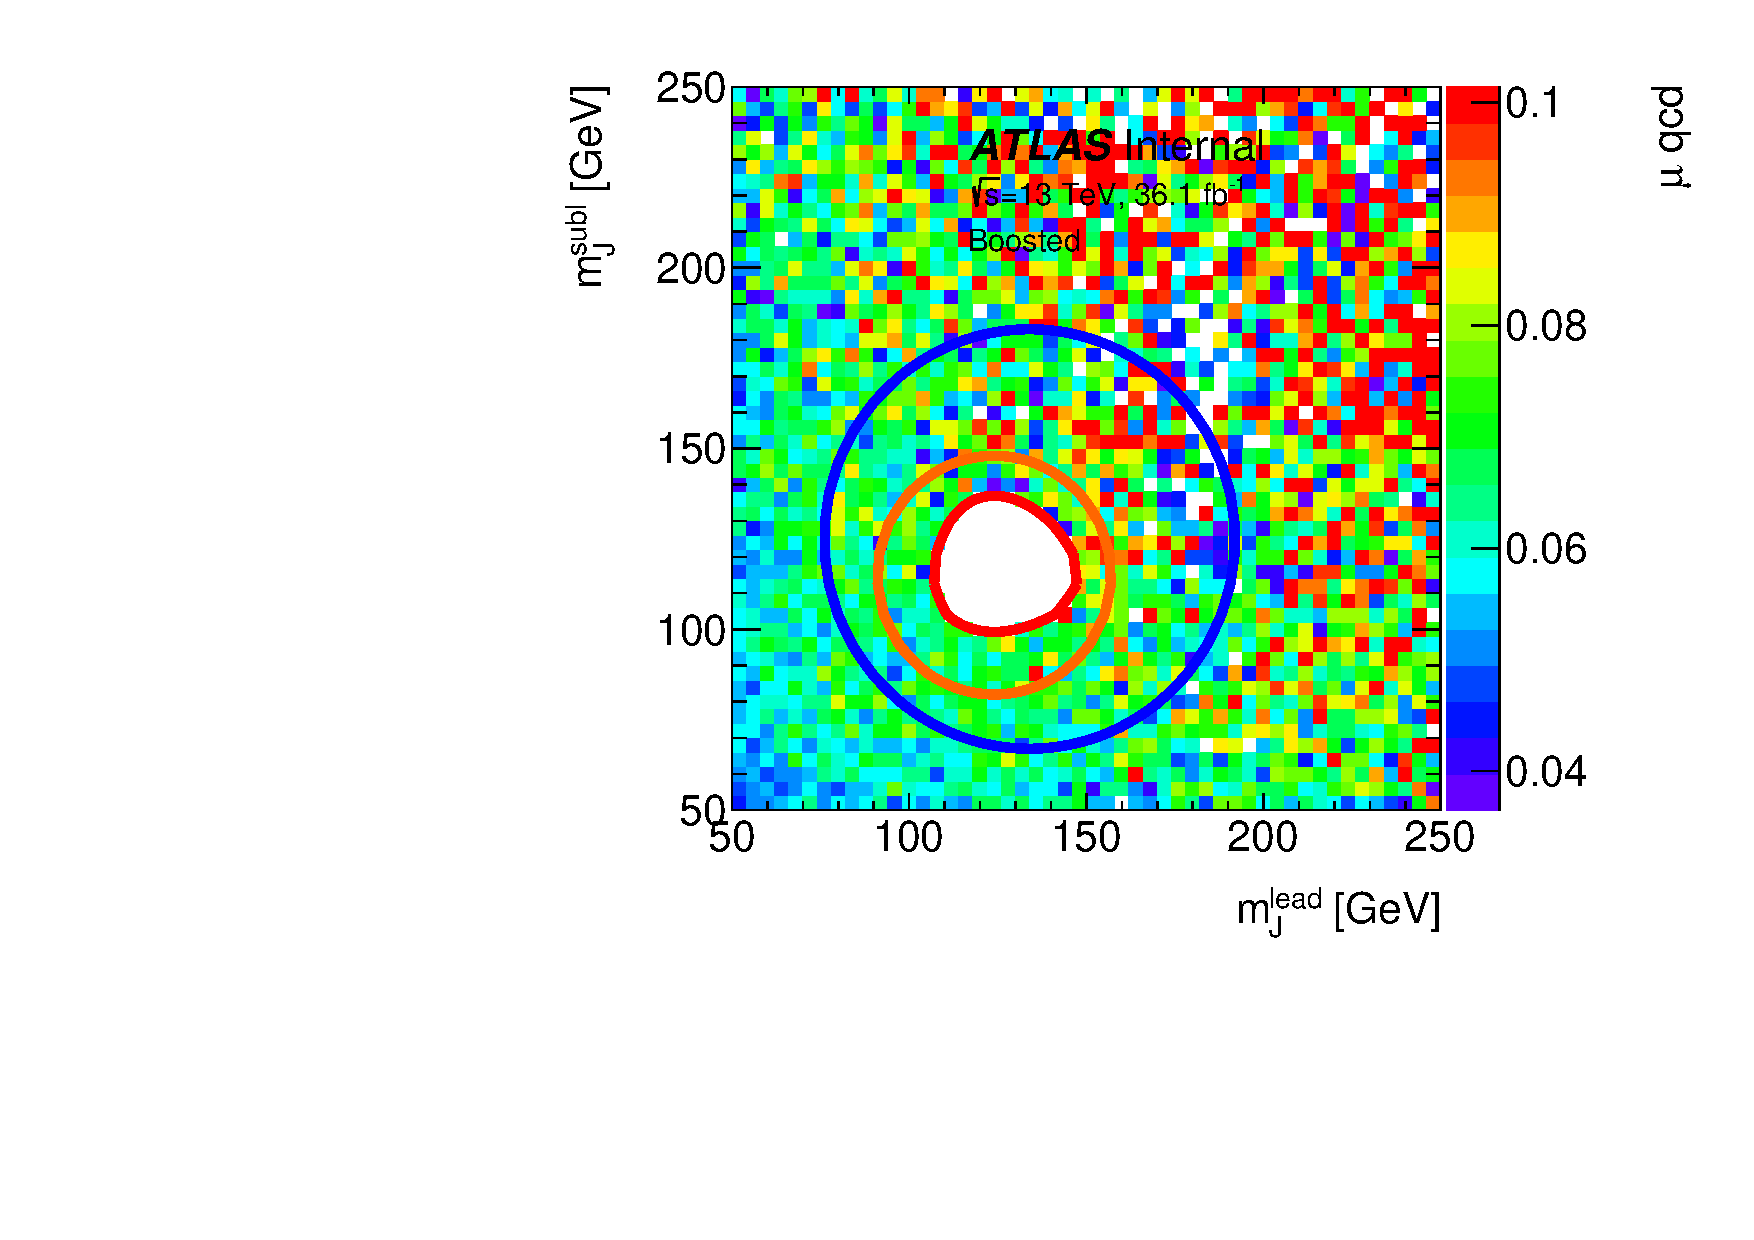
\includegraphics[width=\textwidth,angle=-90]{figures/boosted/AppendixMuqcdstudy/TwoTag_split_Incl_mH0H1.pdf}
        \caption{\muqcd~ on the \mleadJ-\msublJ~ plane}
        \label{fig:app-muqcd-2bs-2d}
    \end{subfigure}
    \quad \quad \quad \quad 
    \begin{subfigure}[b]{0.4\textwidth}
        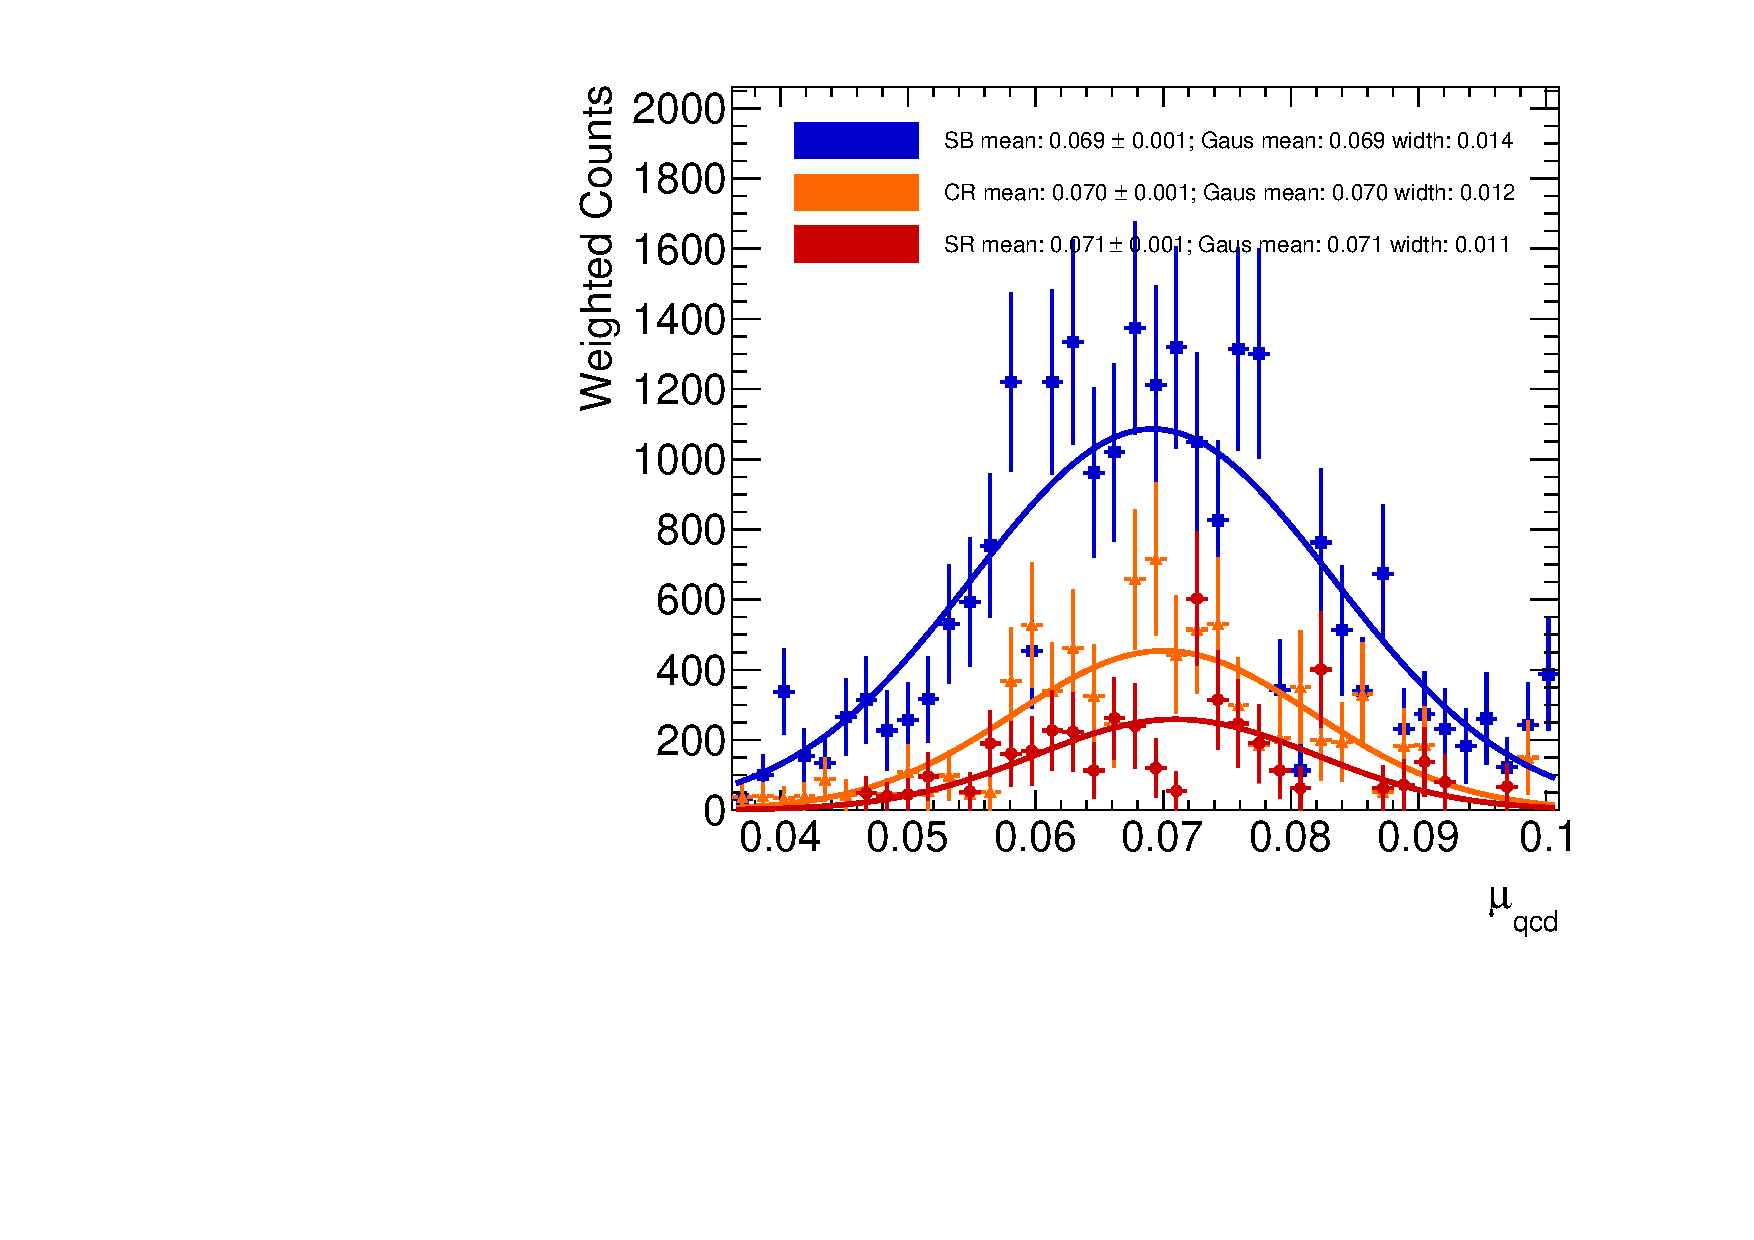
\includegraphics[width=\textwidth,angle=-90]{figures/boosted/AppendixMuqcdstudy/TwoTag_split_Incl_mH0H1_pull.pdf}
        \caption{pulled \muqcd~ distribution in SB/CR/SR}
        \label{fig:app-muqcd-2bs-pull}
    \end{subfigure}
\caption{$2bs$ over $1b$ \muqcd~ values evaluated in data, with the $N_{event}$ weighted mean and the Gaussian fit mean listed.}
\label{fig:app-muqcd-2bs}
\end{figure}

\begin{figure}[htb!]
\centering
\captionsetup{justification=centering}
	\hspace{-1cm}
    \begin{subfigure}[b]{0.4\textwidth}
        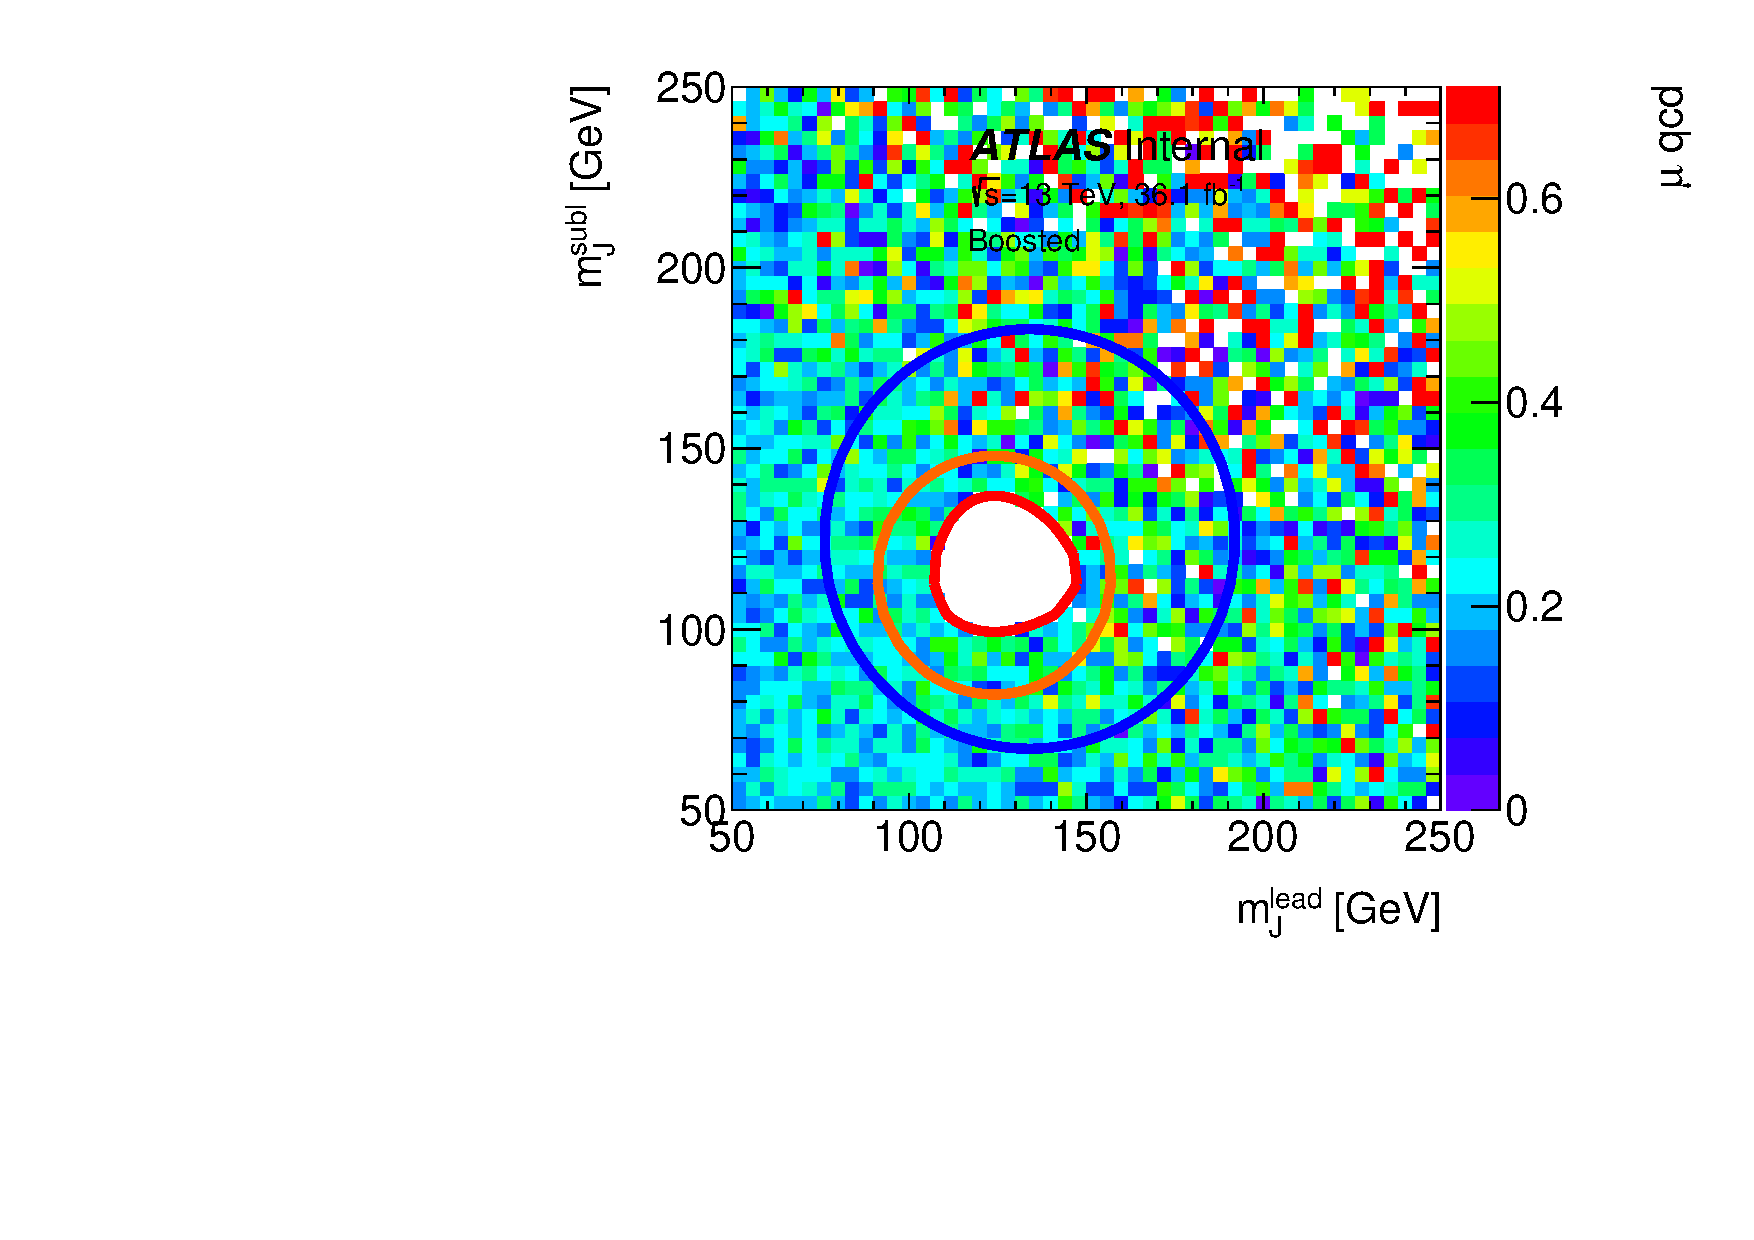
\includegraphics[width=\textwidth,angle=-90]{figures/boosted/AppendixMuqcdstudy/ThreeTag_Incl_mH0H1.pdf}
        \caption{\muqcd~ on the \mleadJ-\msublJ~ plane}
        \label{fig:app-muqcd-3b-2d}
    \end{subfigure}
    \quad \quad \quad \quad 
    \begin{subfigure}[b]{0.4\textwidth}
        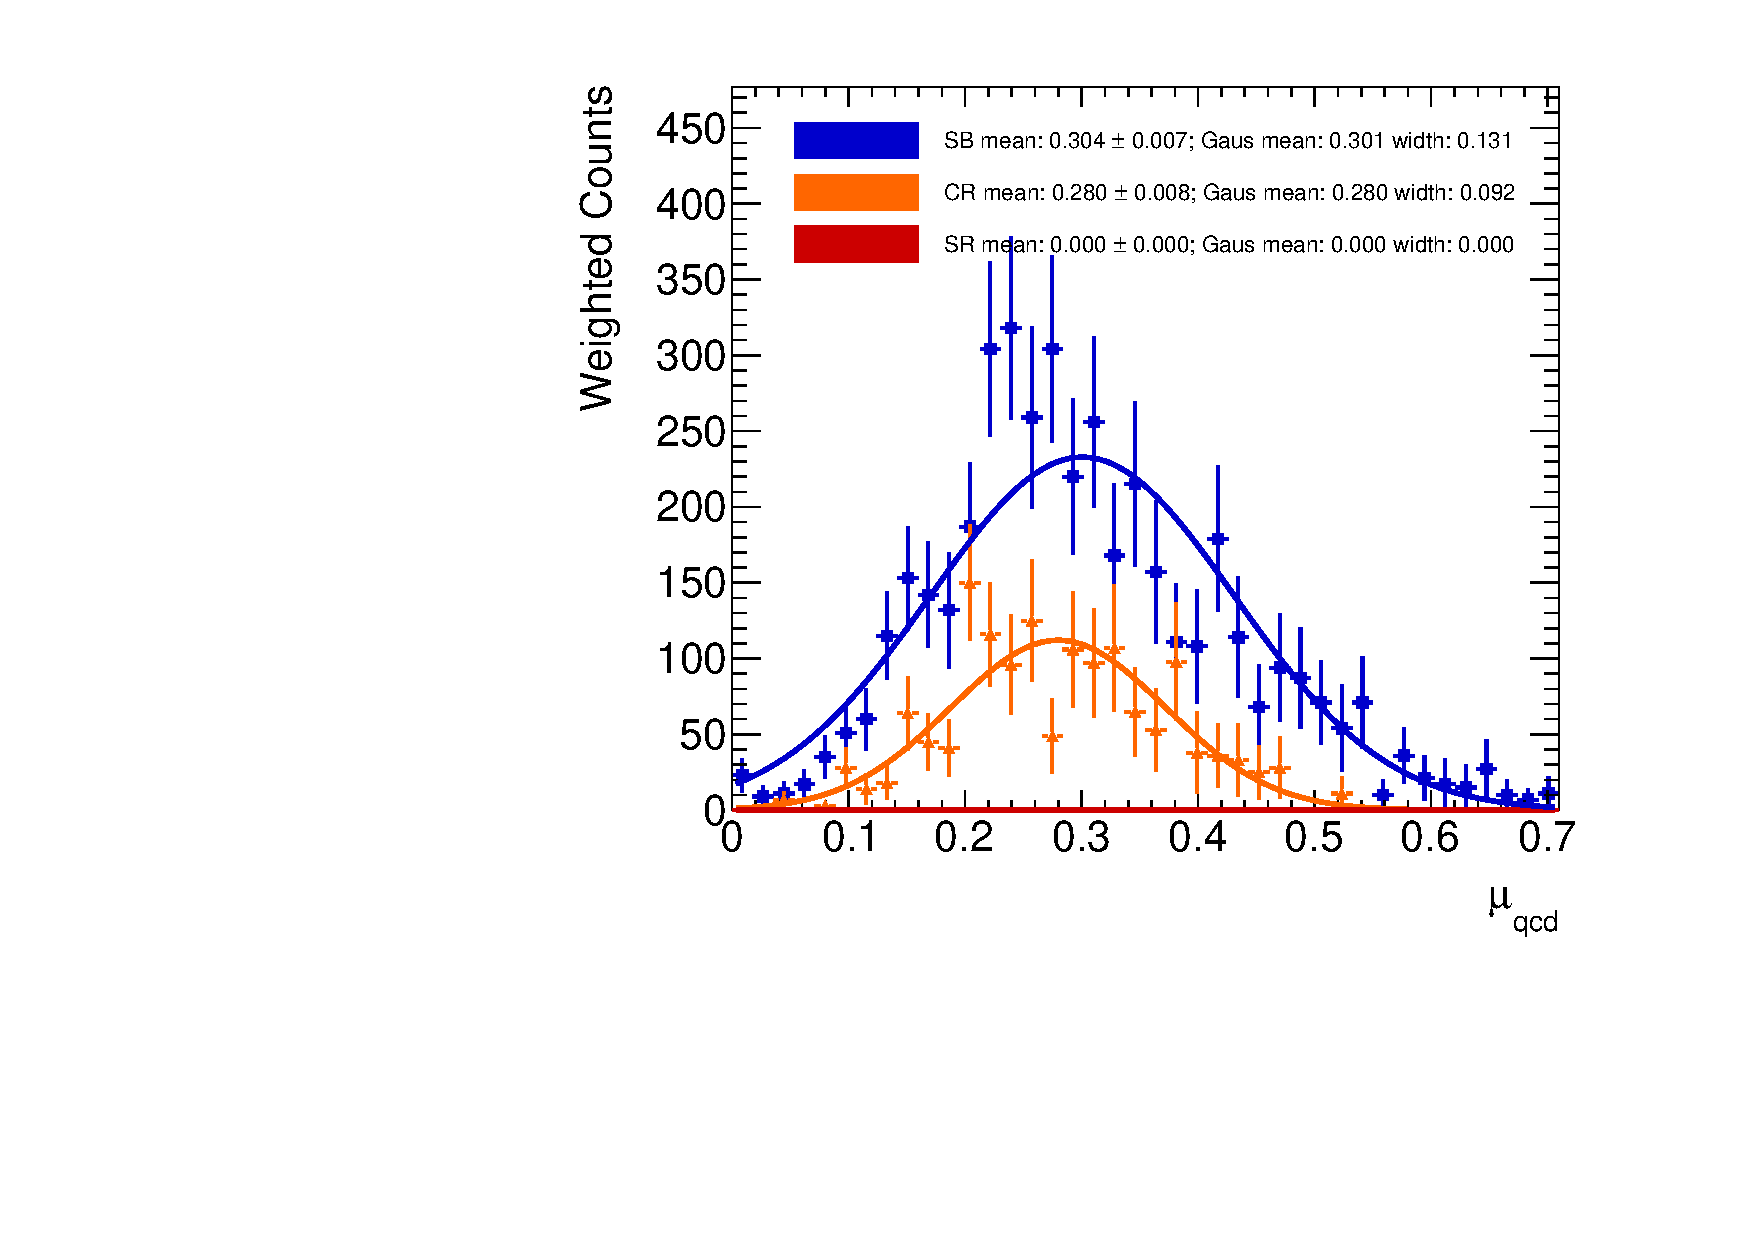
\includegraphics[width=\textwidth,angle=-90]{figures/boosted/AppendixMuqcdstudy/ThreeTag_Incl_mH0H1_pull.pdf}
        \caption{pulled \muqcd~ distribution in SB/CR/SR}
        \label{fig:app-muqcd-3b-pull}
    \end{subfigure}
\caption{$3b$ over $2b$ \muqcd~ values evaluated in data, with the $N_{event}$ weighted mean and the Gaussian fit mean listed. The signal region is blinded.}
\label{fig:app-muqcd-3b}
\end{figure}

\begin{figure}[htb!]
\centering
\captionsetup{justification=centering}
	\hspace{-1cm}
    \begin{subfigure}[b]{0.4\textwidth}
        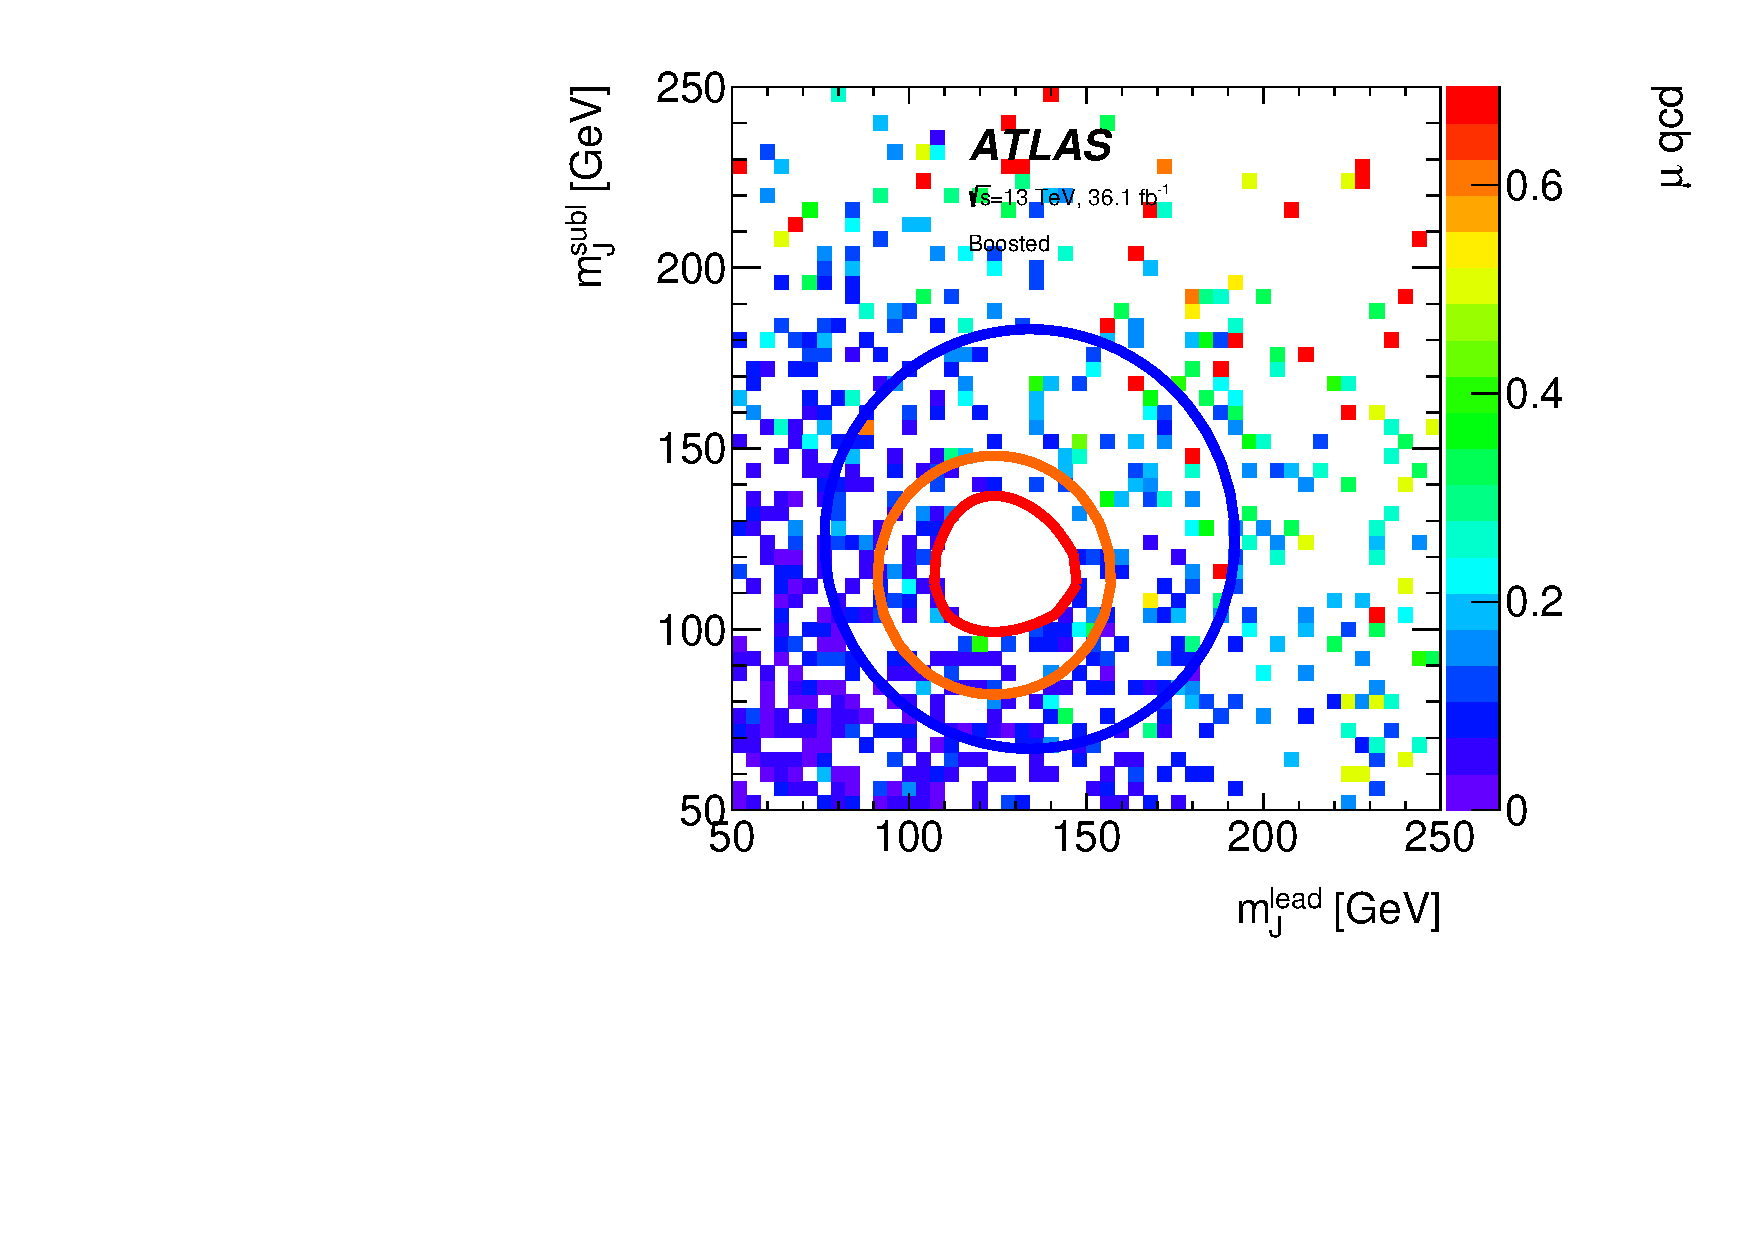
\includegraphics[width=\textwidth,angle=-90]{figures/boosted/AppendixMuqcdstudy/FourTag_Incl_mH0H1.pdf}
        \caption{\muqcd~ on the \mleadJ-\msublJ~ plane}
        \label{fig:app-muqcd-4b-2d}
    \end{subfigure}
    \quad \quad \quad \quad 
    \begin{subfigure}[b]{0.4\textwidth}
        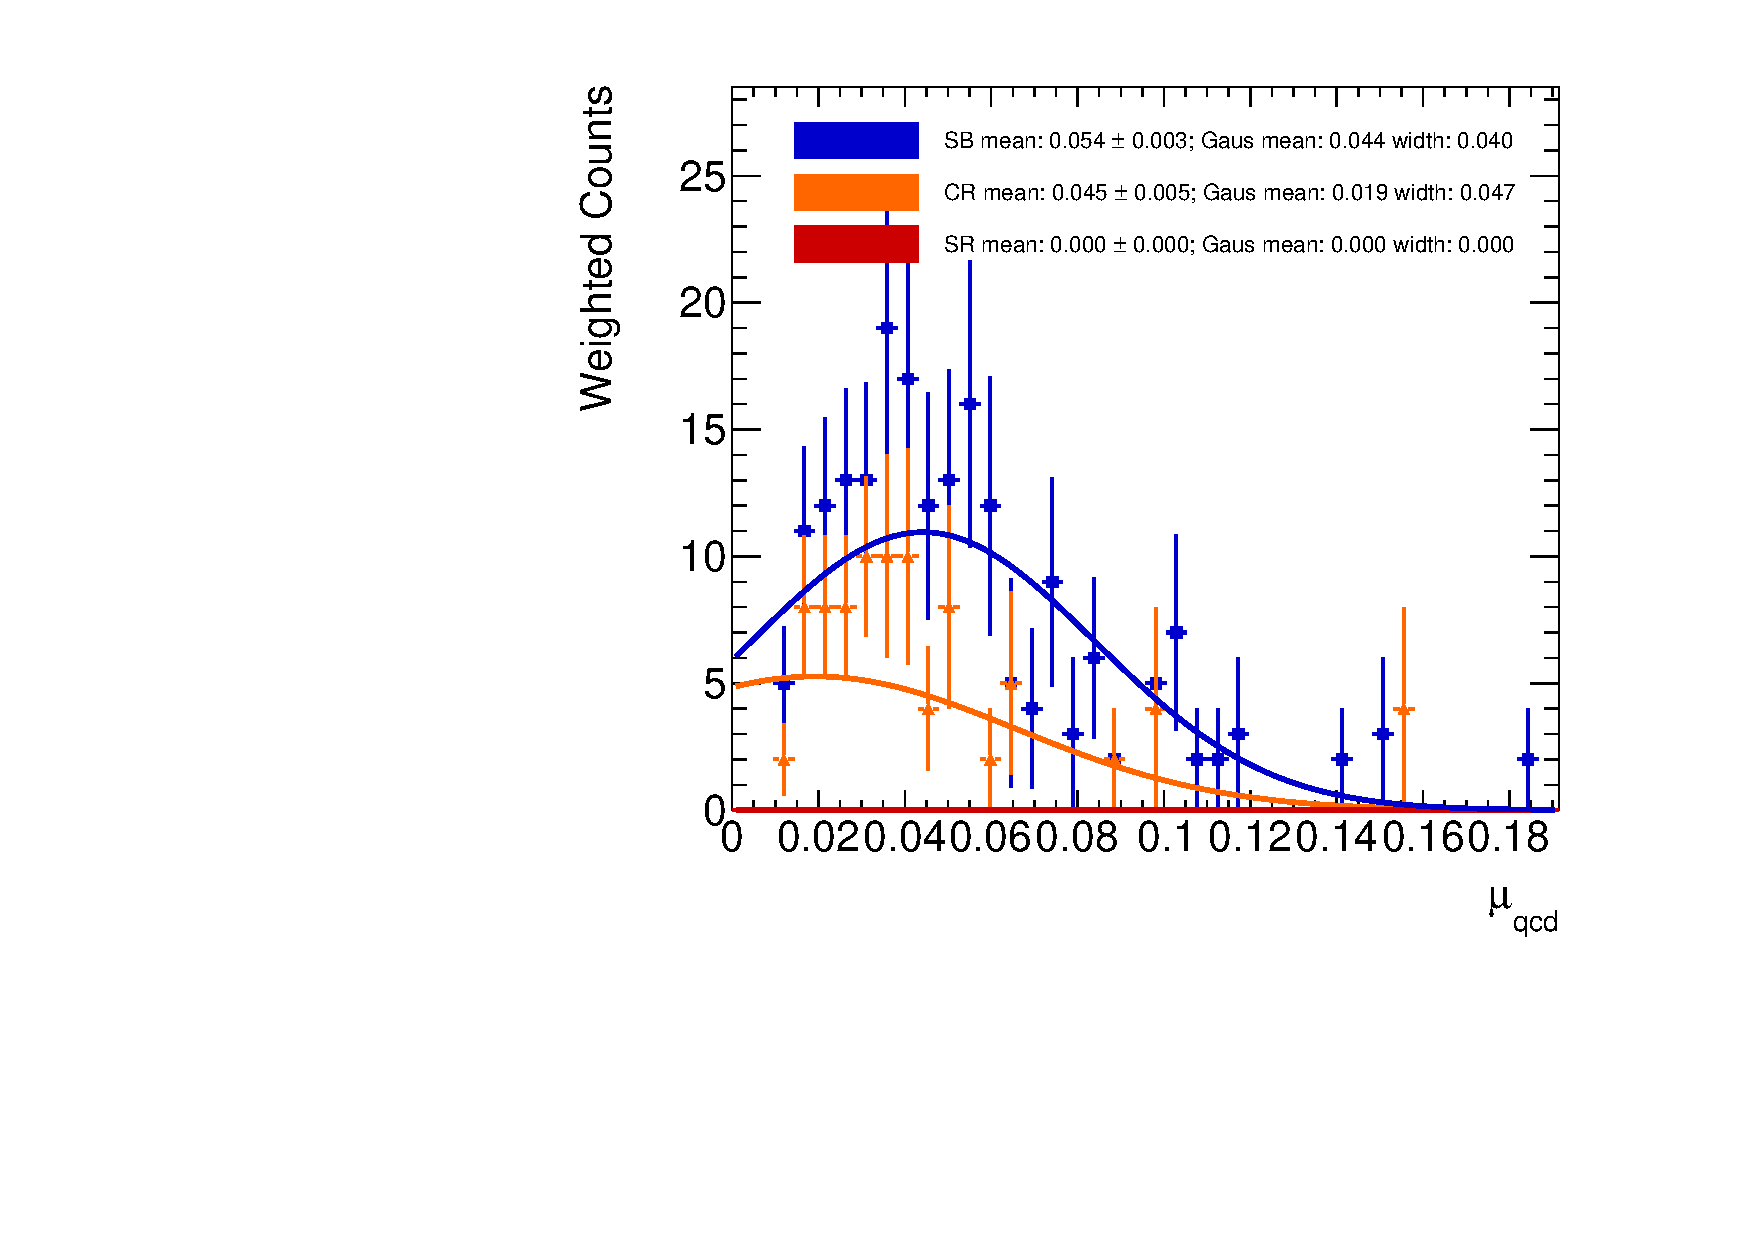
\includegraphics[width=\textwidth,angle=-90]{figures/boosted/AppendixMuqcdstudy/FourTag_Incl_mH0H1_pull.pdf}
        \caption{pulled \muqcd~ distribution in SB/CR/SR}
        \label{fig:app-muqcd-4b-pull}
    \end{subfigure}
\caption{$4b$ over $2b$ \muqcd~ values evaluated in data, with the $N_{event}$ weighted mean and the Gaussian fit mean listed. The signal region is blinded.}
\label{fig:app-muqcd-4b}
\end{figure}

\paragraph{}
Also, the dijet MC can be used for constant \muqcd~ validation. 
The same distributions evaluated in dijet MC are shown in Figure~\ref{fig:app-muqcd-1b-qcd} ($1b$ over $0b$), ~\ref{fig:app-muqcd-2b-qcd} ($2b$ over $1b$), ~\ref{fig:app-muqcd-2bs-qcd} ($2bs$ over $1b$), ~\ref{fig:app-muqcd-3b-qcd} ($3b$ over $2b$), ~\ref{fig:app-muqcd-4b-qcd} ($4b$ over $2b$).  
Poor statistics of the dijet MC samples affects the pull distributions, especially in $3b$ and $4b$, yet the consistency of \muqcd in SB/CR/SR is still validated.
The large difference in \muqcd between data and MC also shows that the dijet MC should not be used directly for background estimation.

\begin{figure}[htb!]
\centering
\captionsetup{justification=centering}
	\hspace{-1cm}
    \begin{subfigure}[b]{0.4\textwidth}
        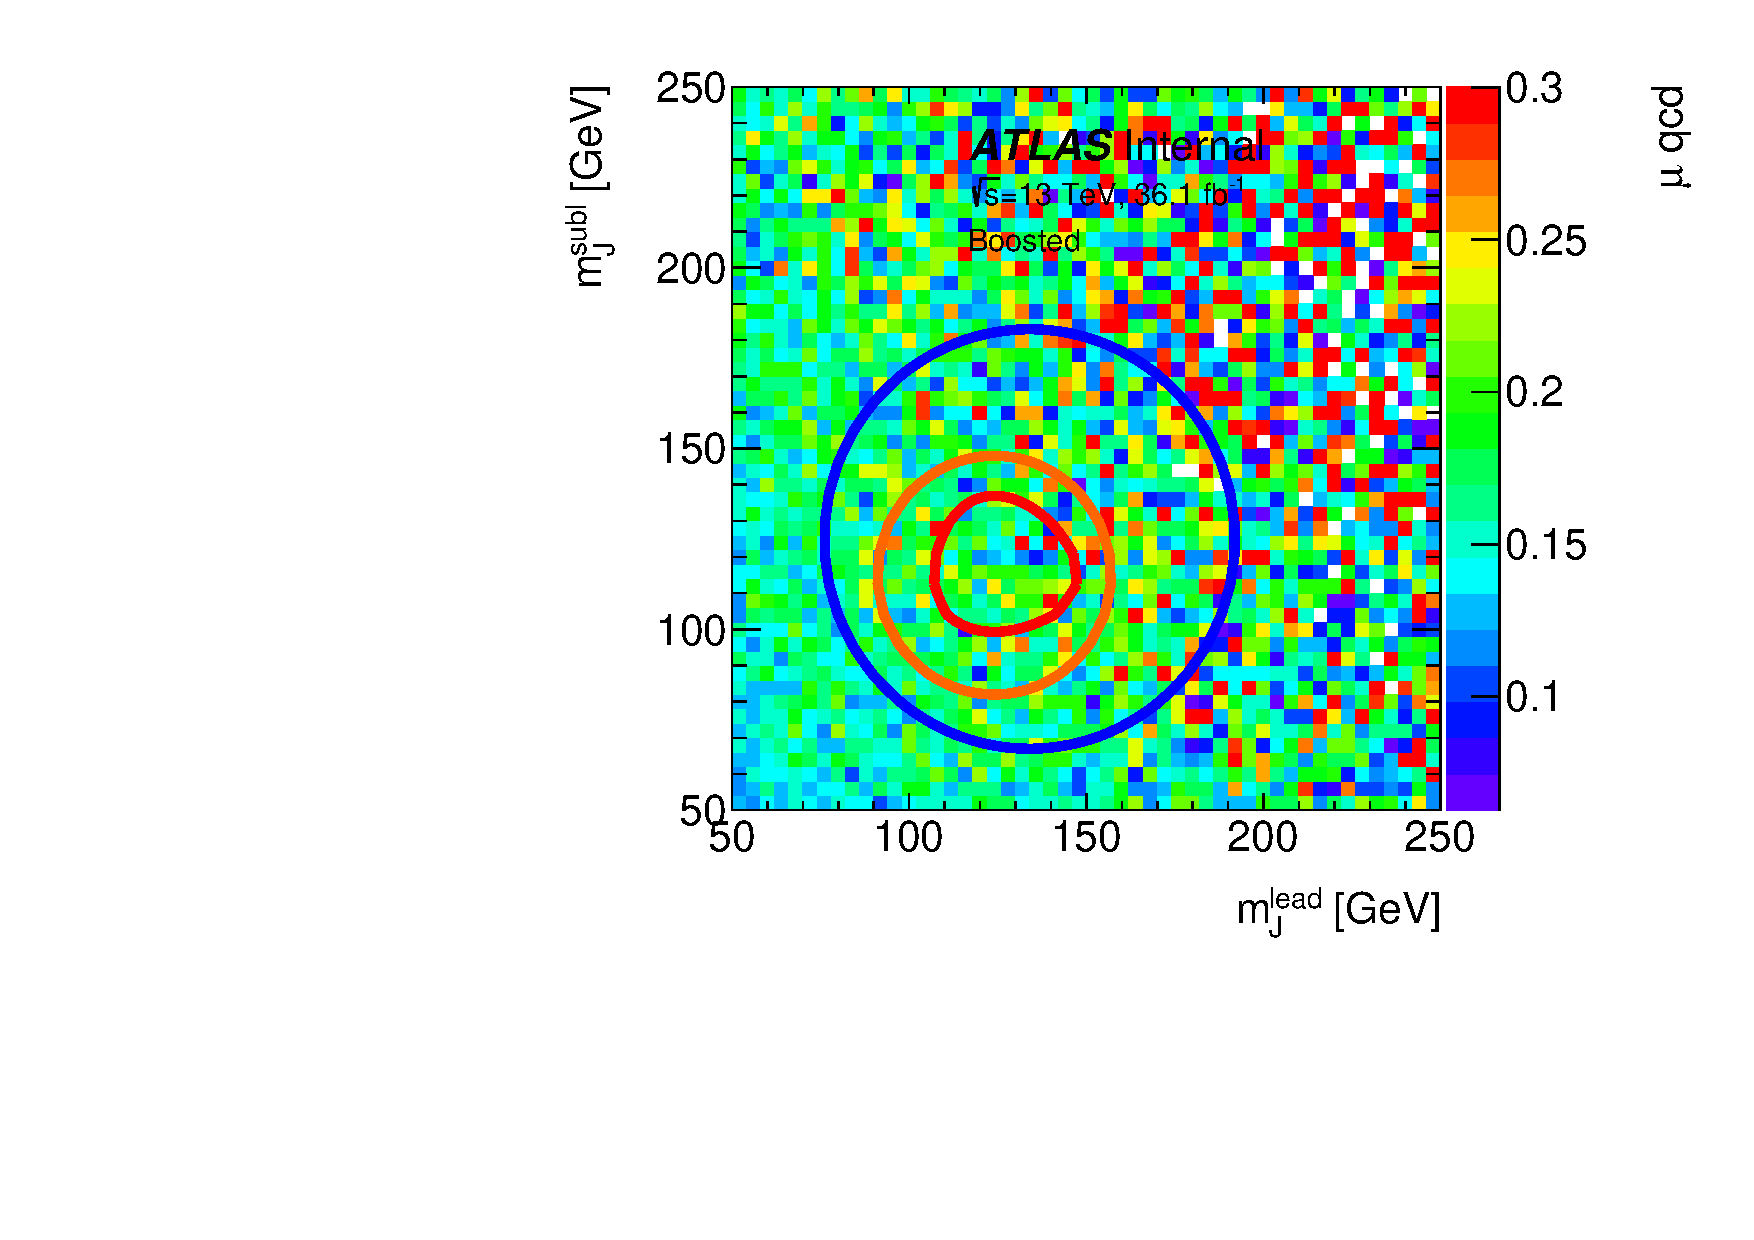
\includegraphics[width=\textwidth,angle=-90]{figures/boosted/AppendixMuqcdstudy/QCD_OneTag_Incl_mH0H1.pdf}
        \caption{\muqcd~ on the \mleadJ-\msublJ~ plane}
        \label{fig:app-muqcd-1b-2d-qcd}
    \end{subfigure}
    \quad \quad \quad \quad 
    \begin{subfigure}[b]{0.4\textwidth}
        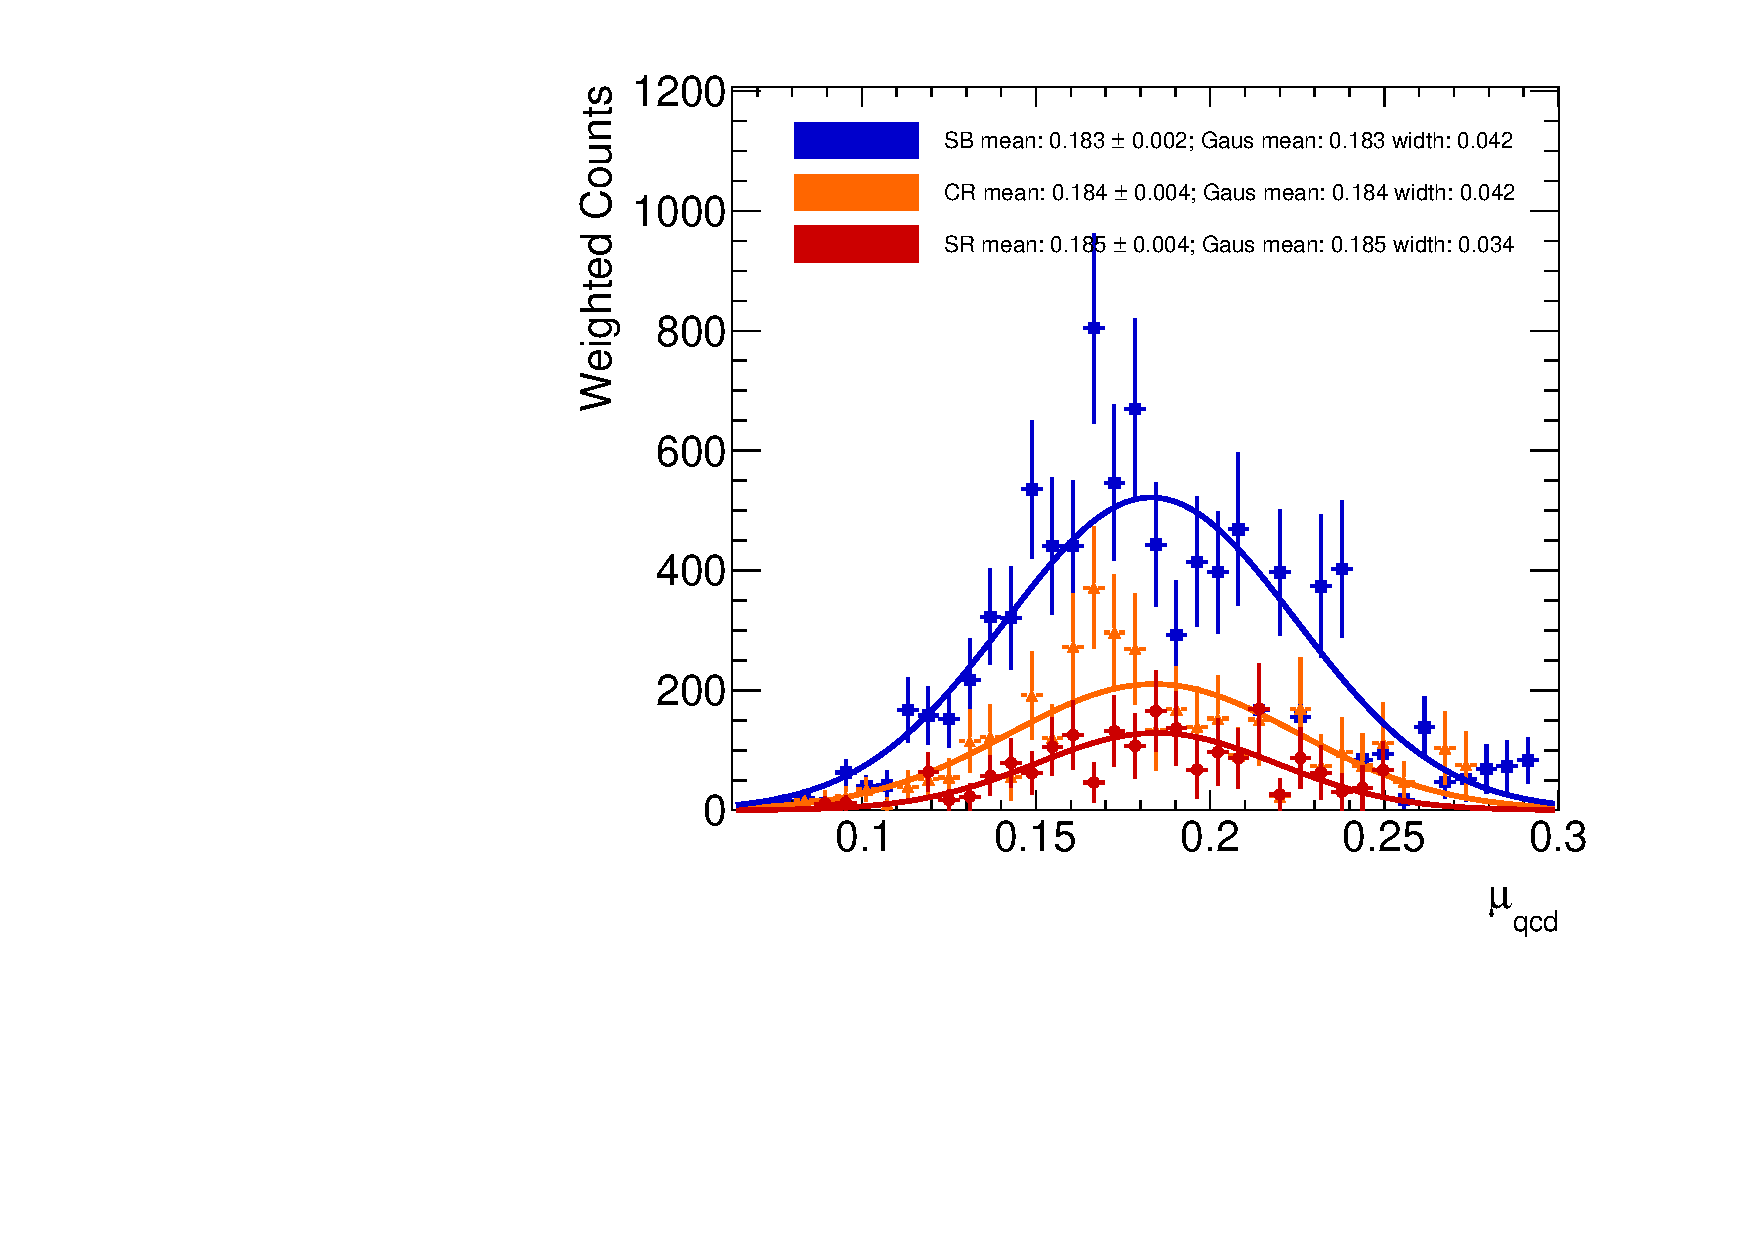
\includegraphics[width=\textwidth,angle=-90]{figures/boosted/AppendixMuqcdstudy/QCD_OneTag_Incl_mH0H1_pull.pdf}
        \caption{pulled \muqcd~ distribution in SB/CR/SR}
        \label{fig:app-muqcd-1b-pull-qcd}
    \end{subfigure}
\caption{$1b$ over $0b$ \muqcd~ values evaluated in dijet MC, with the $N_{event}$ weighted mean and the Gaussian fit mean listed.}
\label{fig:app-muqcd-1b-qcd}
\end{figure}

\begin{figure}[htb!]
\centering
\captionsetup{justification=centering}
	\hspace{-1cm}
    \begin{subfigure}[b]{0.4\textwidth}
        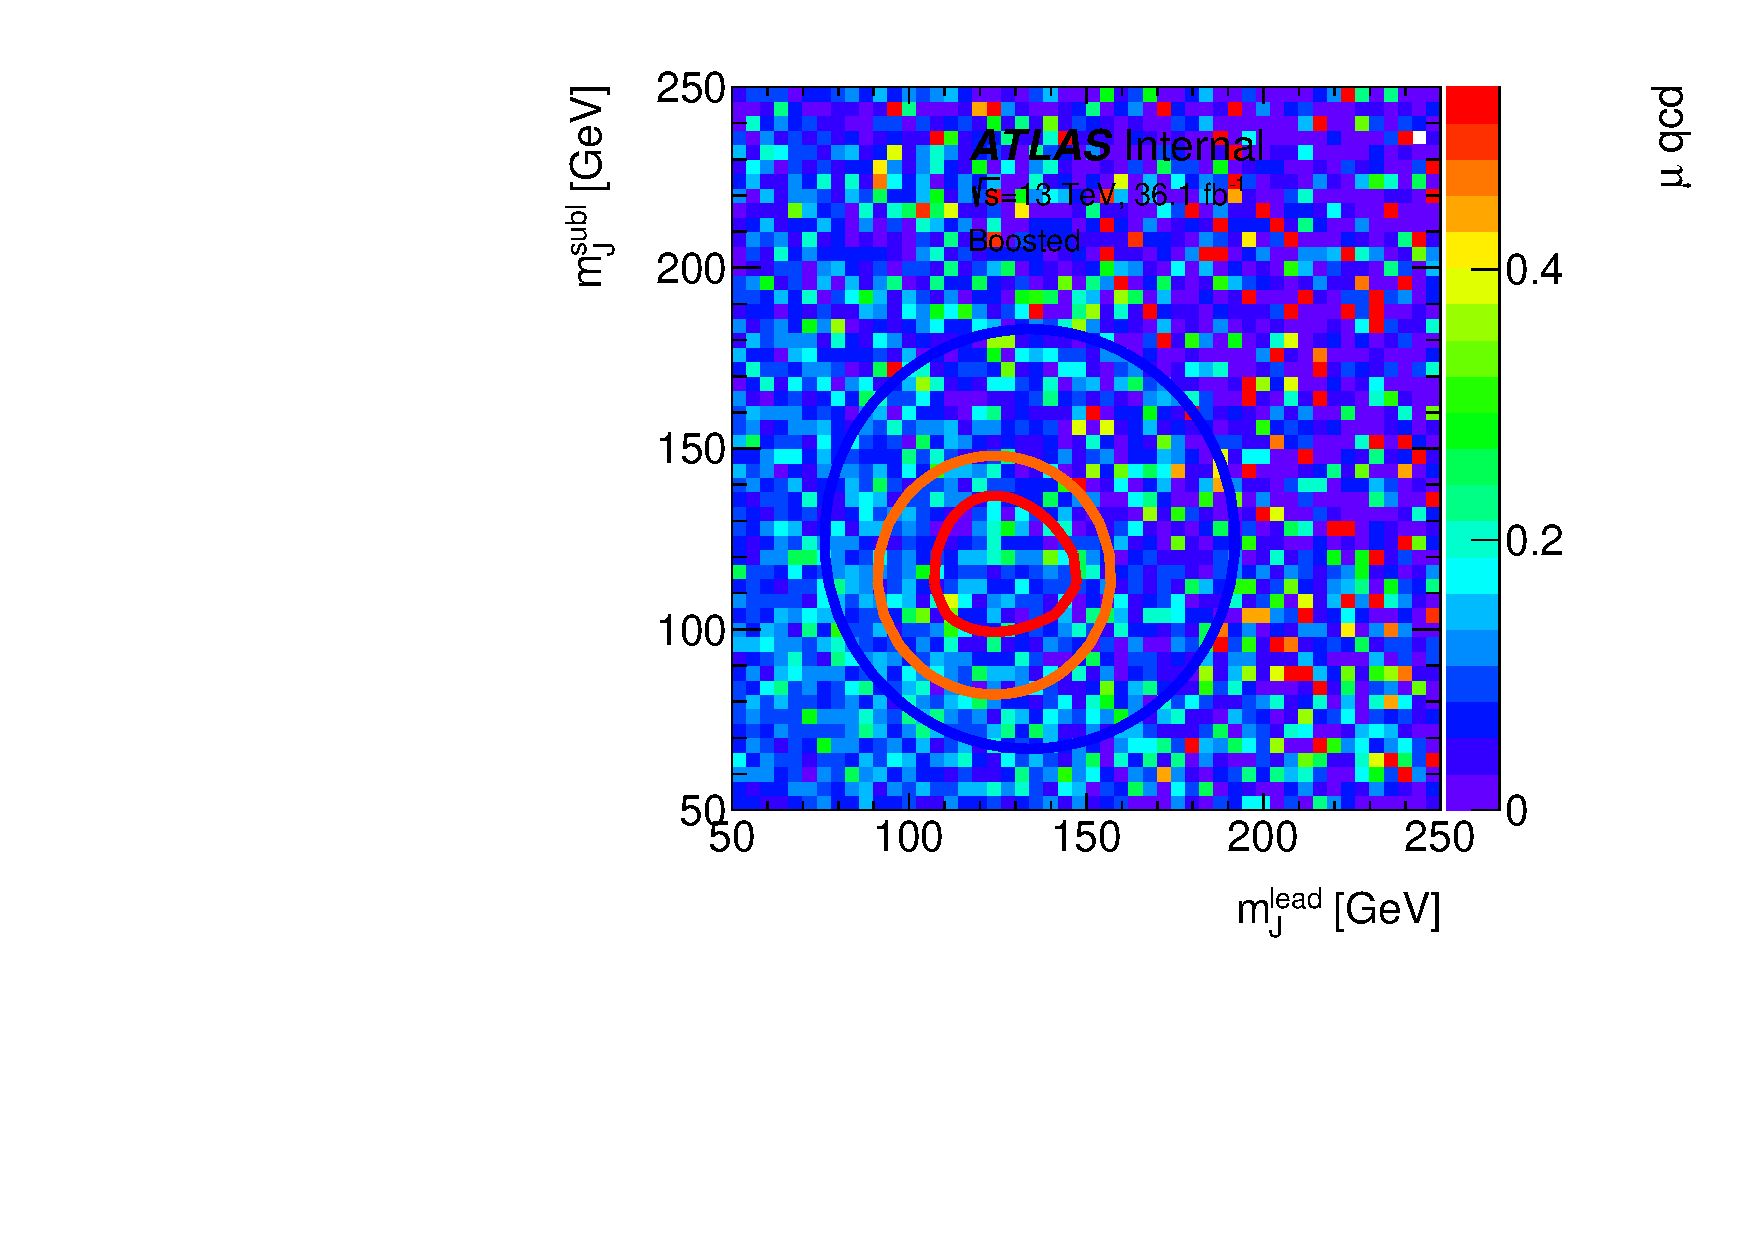
\includegraphics[width=\textwidth,angle=-90]{figures/boosted/AppendixMuqcdstudy/QCD_TwoTag_Incl_mH0H1.pdf}
        \caption{\muqcd~ on the \mleadJ-\msublJ~ plane}
        \label{fig:app-muqcd-2b-2d-qcd}
    \end{subfigure}
    \quad \quad \quad \quad 
    \begin{subfigure}[b]{0.4\textwidth}
        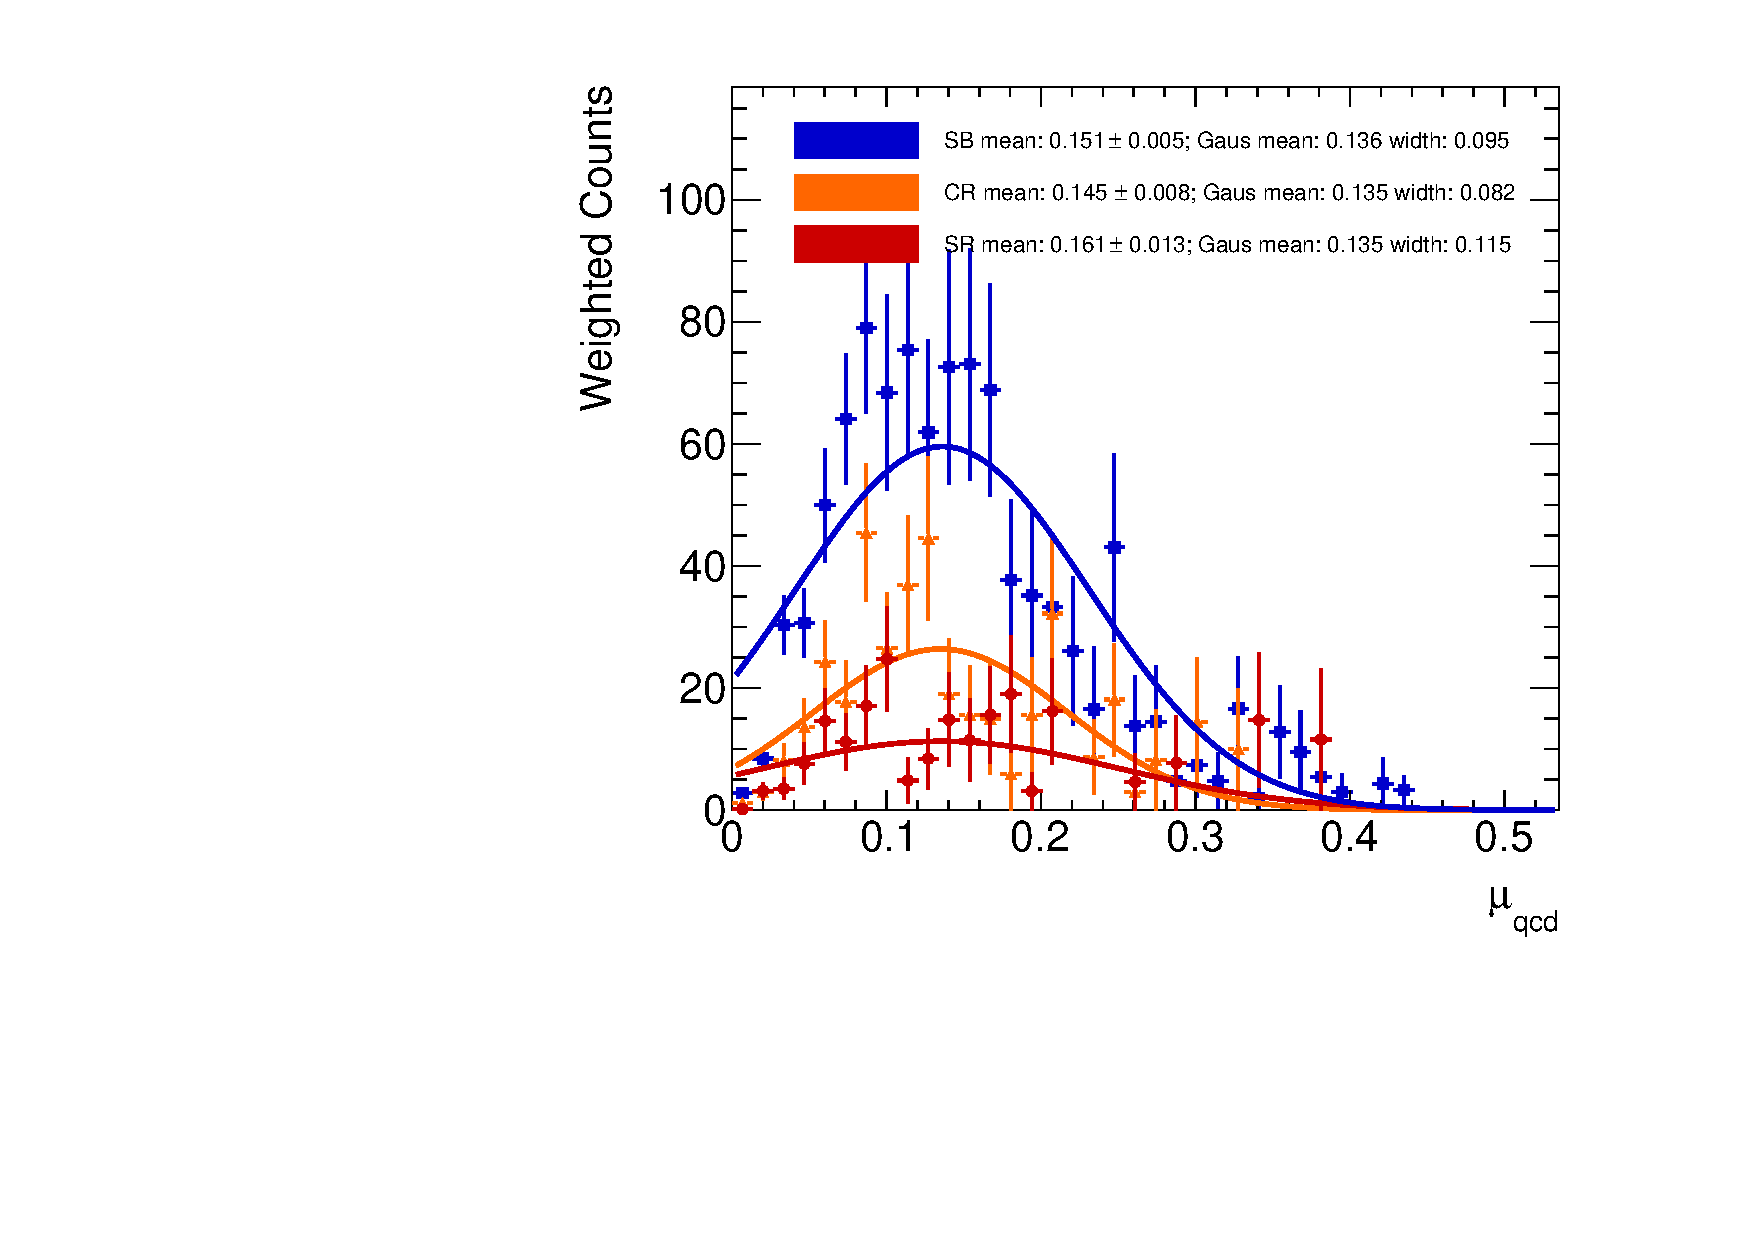
\includegraphics[width=\textwidth,angle=-90]{figures/boosted/AppendixMuqcdstudy/QCD_TwoTag_Incl_mH0H1_pull.pdf}
        \caption{pulled \muqcd~ distribution in SB/CR/SR}
        \label{fig:app-muqcd-2b-pull-qcd}
    \end{subfigure}
\caption{$2b$ over $1b$ \muqcd~ values evaluated in dijet MC, with the $N_{event}$ weighted mean and the Gaussian fit mean listed.}
\label{fig:app-muqcd-2b-qcd}
\end{figure}

\begin{figure}[htb!]
\centering
\captionsetup{justification=centering}
	\hspace{-1cm}
    \begin{subfigure}[b]{0.4\textwidth}
        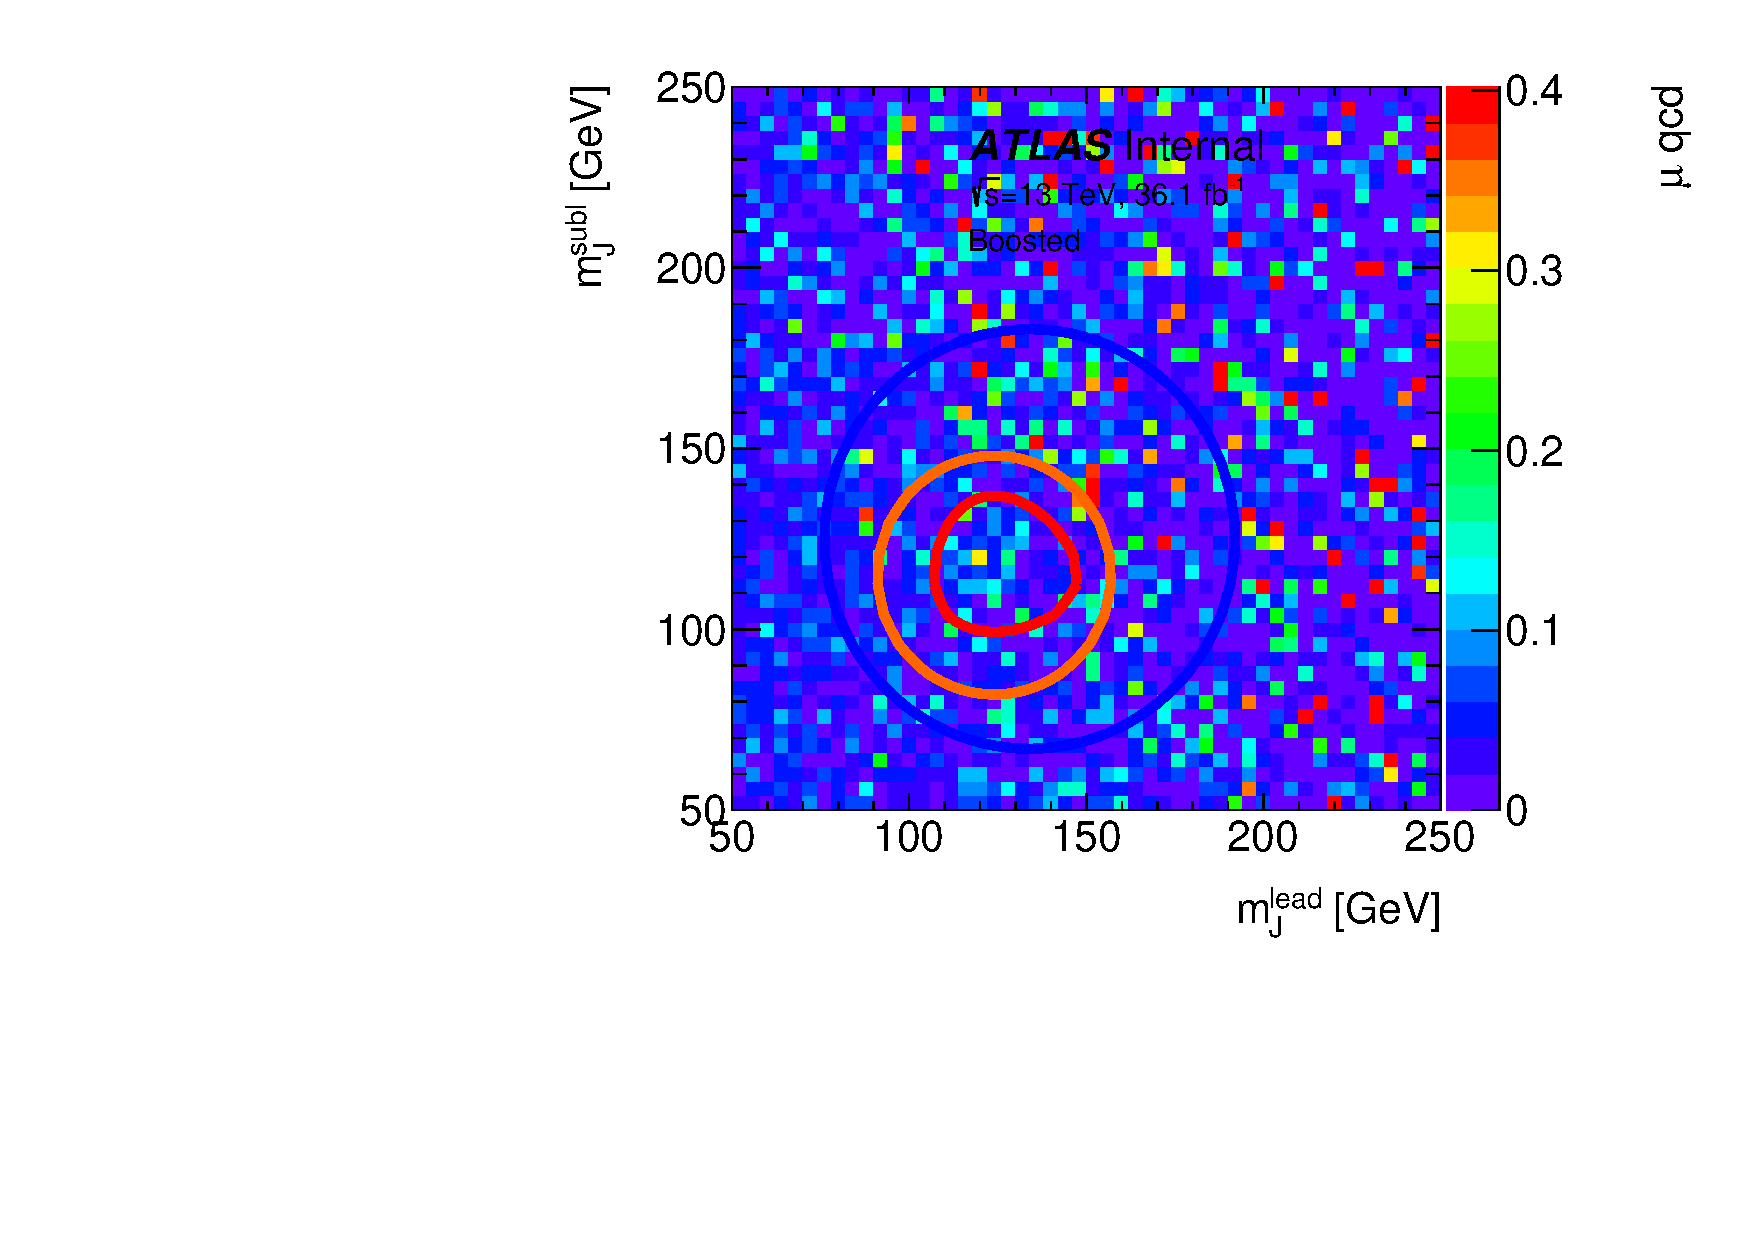
\includegraphics[width=\textwidth,angle=-90]{figures/boosted/AppendixMuqcdstudy/QCD_TwoTag_split_Incl_mH0H1.pdf}
        \caption{\muqcd~ on the \mleadJ-\msublJ~ plane}
        \label{fig:app-muqcd-2bs-2d-qcd}
    \end{subfigure}
    \quad \quad \quad \quad 
    \begin{subfigure}[b]{0.4\textwidth}
        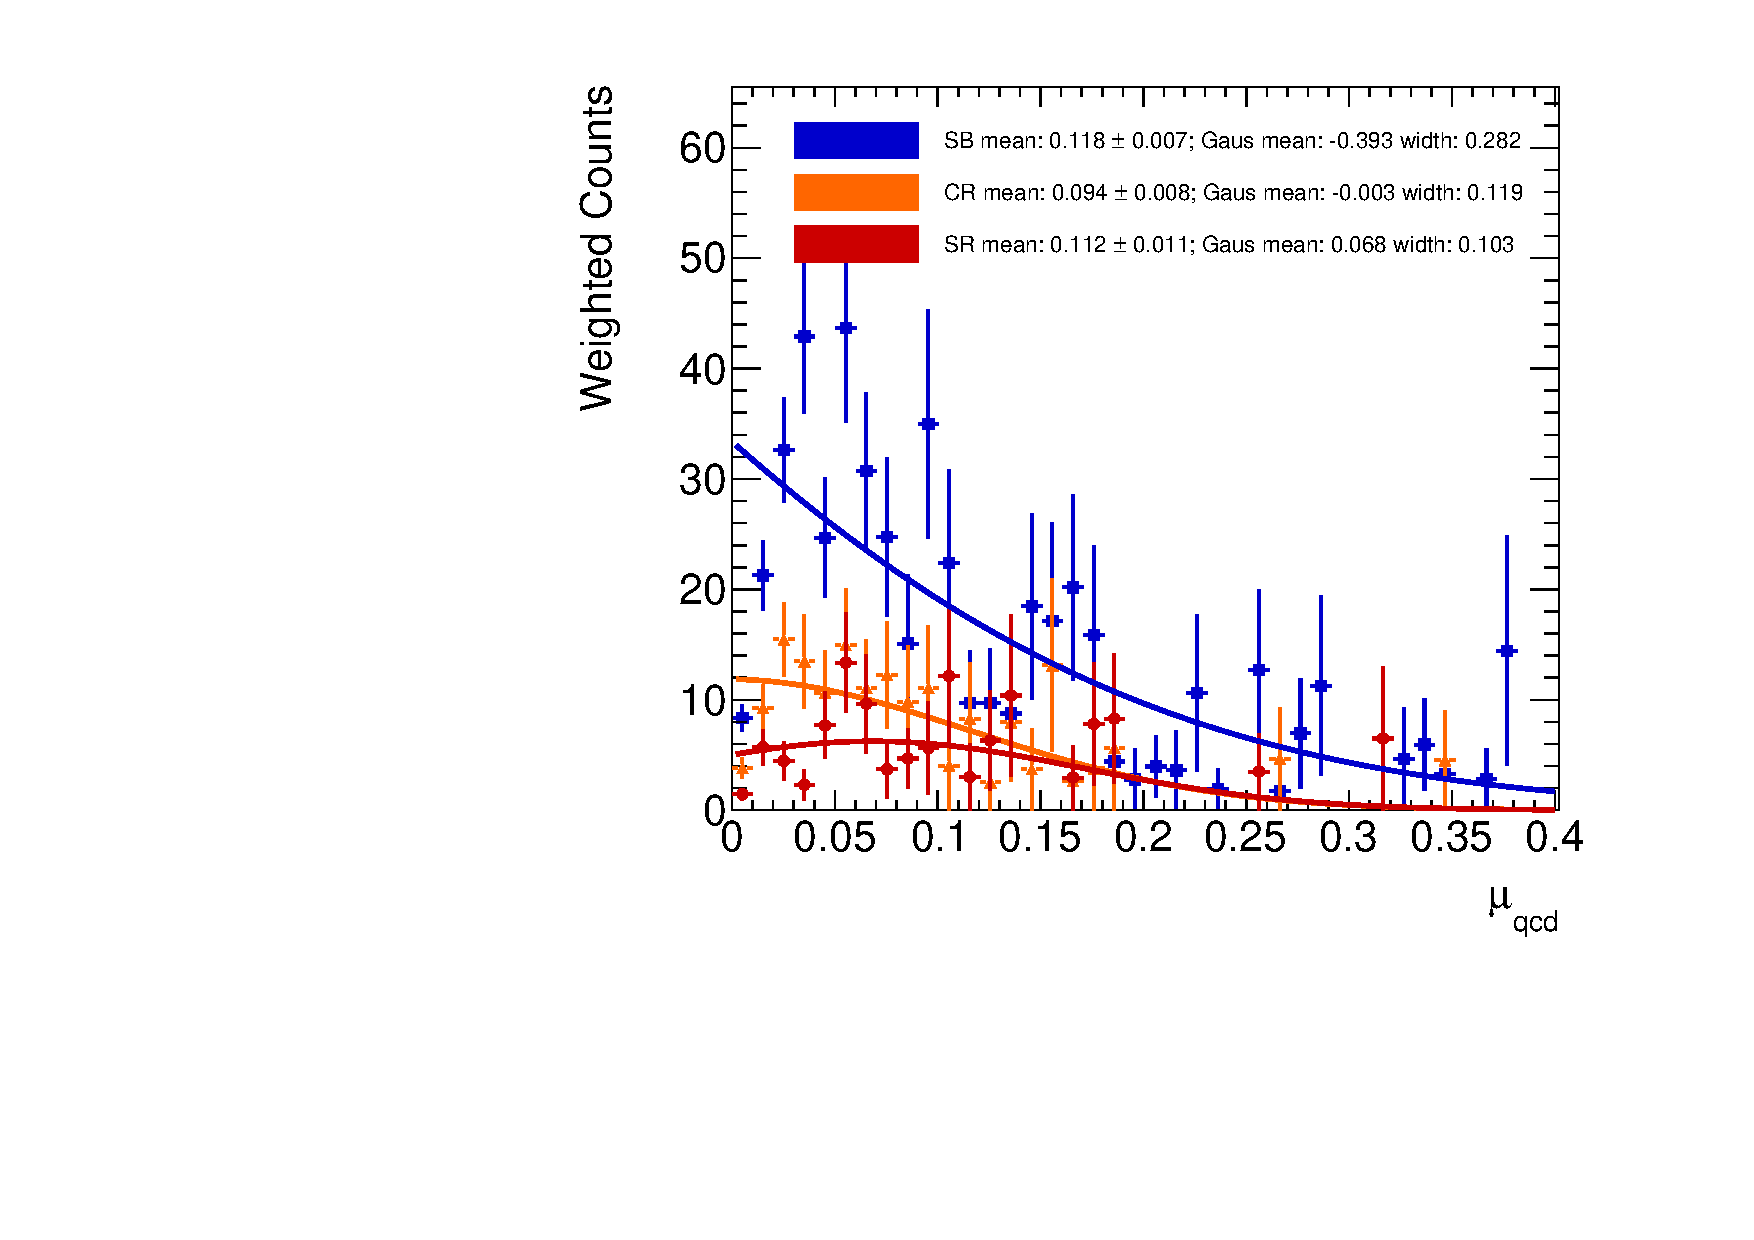
\includegraphics[width=\textwidth,angle=-90]{figures/boosted/AppendixMuqcdstudy/QCD_TwoTag_split_Incl_mH0H1_pull.pdf}
        \caption{pulled \muqcd~ distribution in SB/CR/SR}
        \label{fig:app-muqcd-2bs-pull-qcd}
    \end{subfigure}
\caption{$2bs$ over $1b$ \muqcd~ values evaluated in dijet MC, with the $N_{event}$ weighted mean and the Gaussian fit mean listed.}
\label{fig:app-muqcd-2bs-qcd}
\end{figure}

\begin{figure}[htb!]
\centering
\captionsetup{justification=centering}
	\hspace{-1cm}
    \begin{subfigure}[b]{0.4\textwidth}
        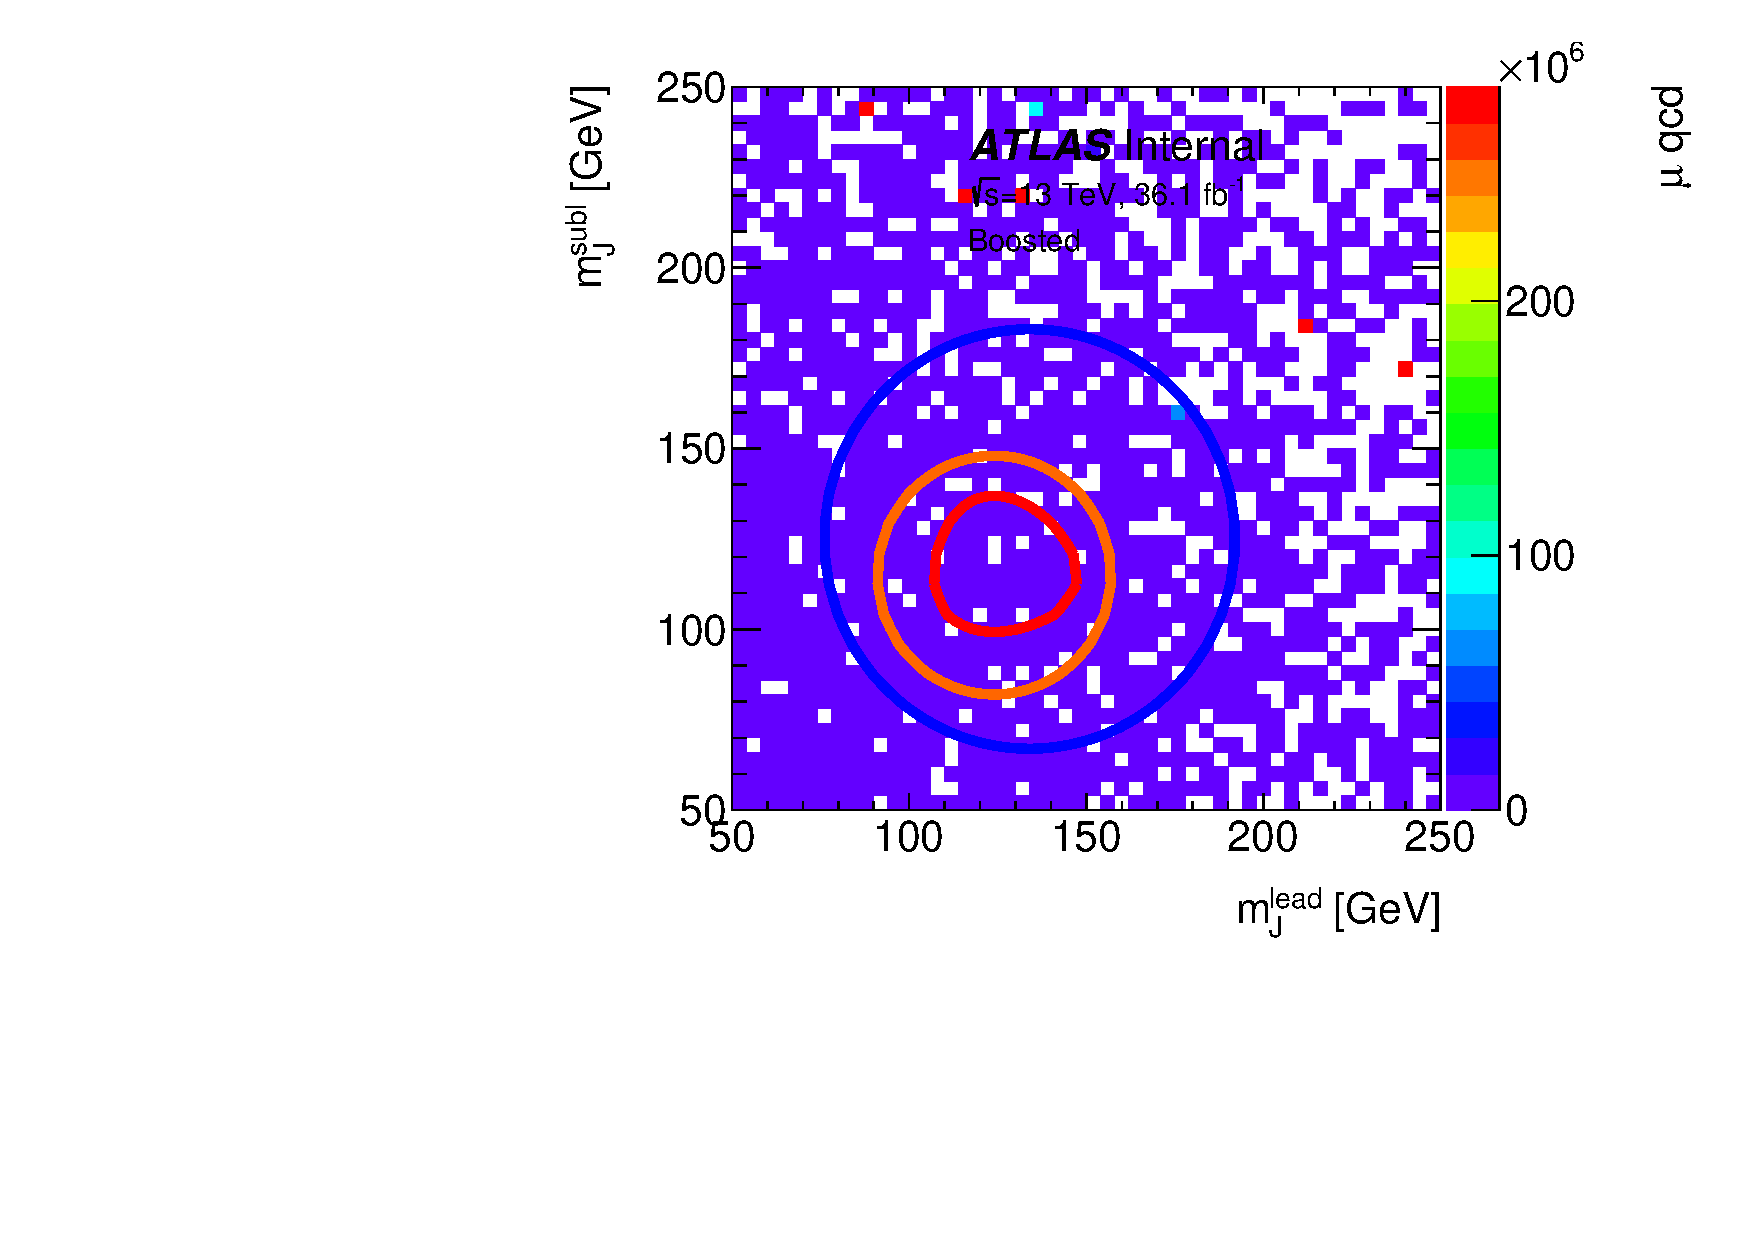
\includegraphics[width=\textwidth,angle=-90]{figures/boosted/AppendixMuqcdstudy/QCD_ThreeTag_Incl_mH0H1.pdf}
        \caption{\muqcd~ on the \mleadJ-\msublJ~ plane}
        \label{fig:app-muqcd-3b-2d-qcd}
    \end{subfigure}
    \quad \quad \quad \quad 
    \begin{subfigure}[b]{0.4\textwidth}
        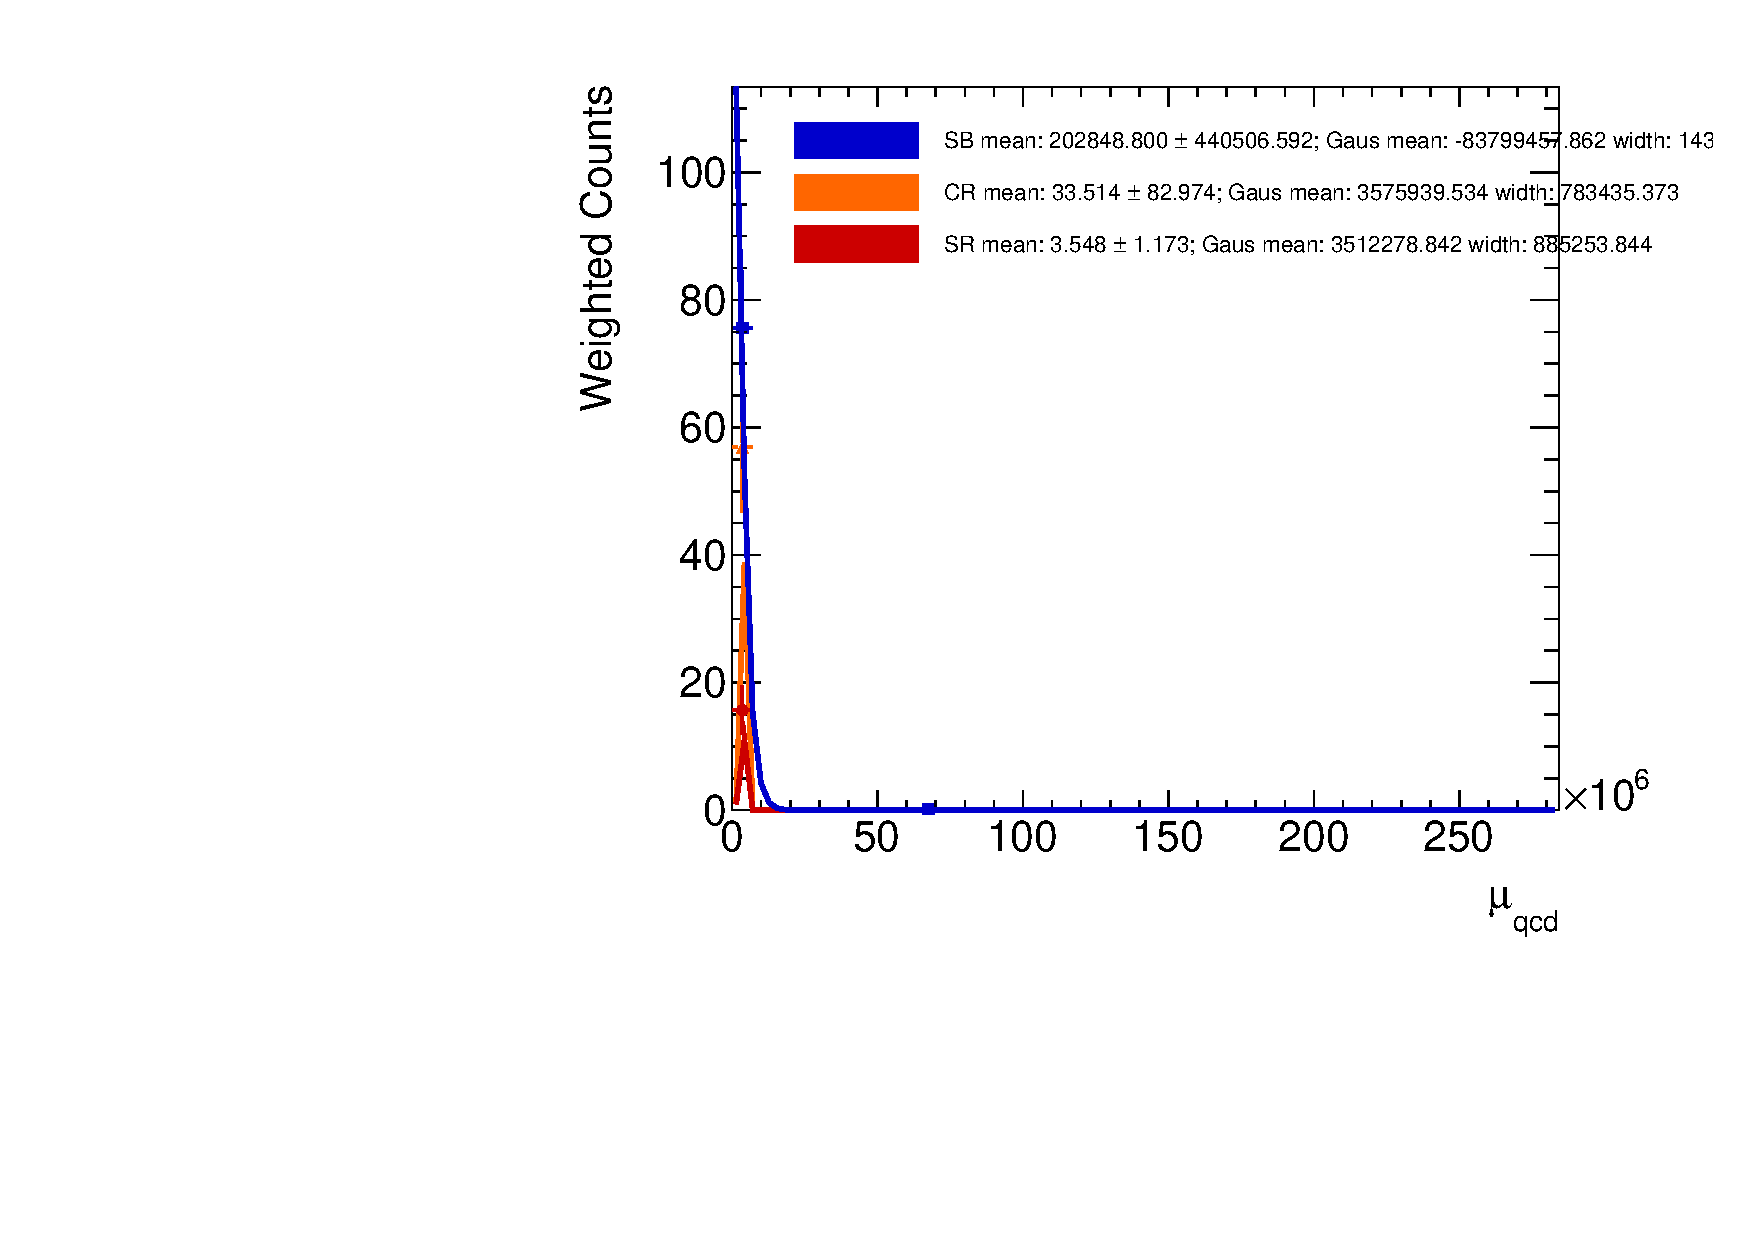
\includegraphics[width=\textwidth,angle=-90]{figures/boosted/AppendixMuqcdstudy/QCD_ThreeTag_Incl_mH0H1_pull.pdf}
        \caption{pulled \muqcd~ distribution in SB/CR/SR}
        \label{fig:app-muqcd-3b-pull-qcd}
    \end{subfigure}
\caption{$3b$ over $2b$ \muqcd~ values evaluated in dijet MC, with the $N_{event}$ weighted mean and the Gaussian fit mean listed.}
\label{fig:app-muqcd-3b-qcd}
\end{figure}

\begin{figure}[htb!]
\centering
\captionsetup{justification=centering}
	\hspace{-1cm}
    \begin{subfigure}[b]{0.4\textwidth}
        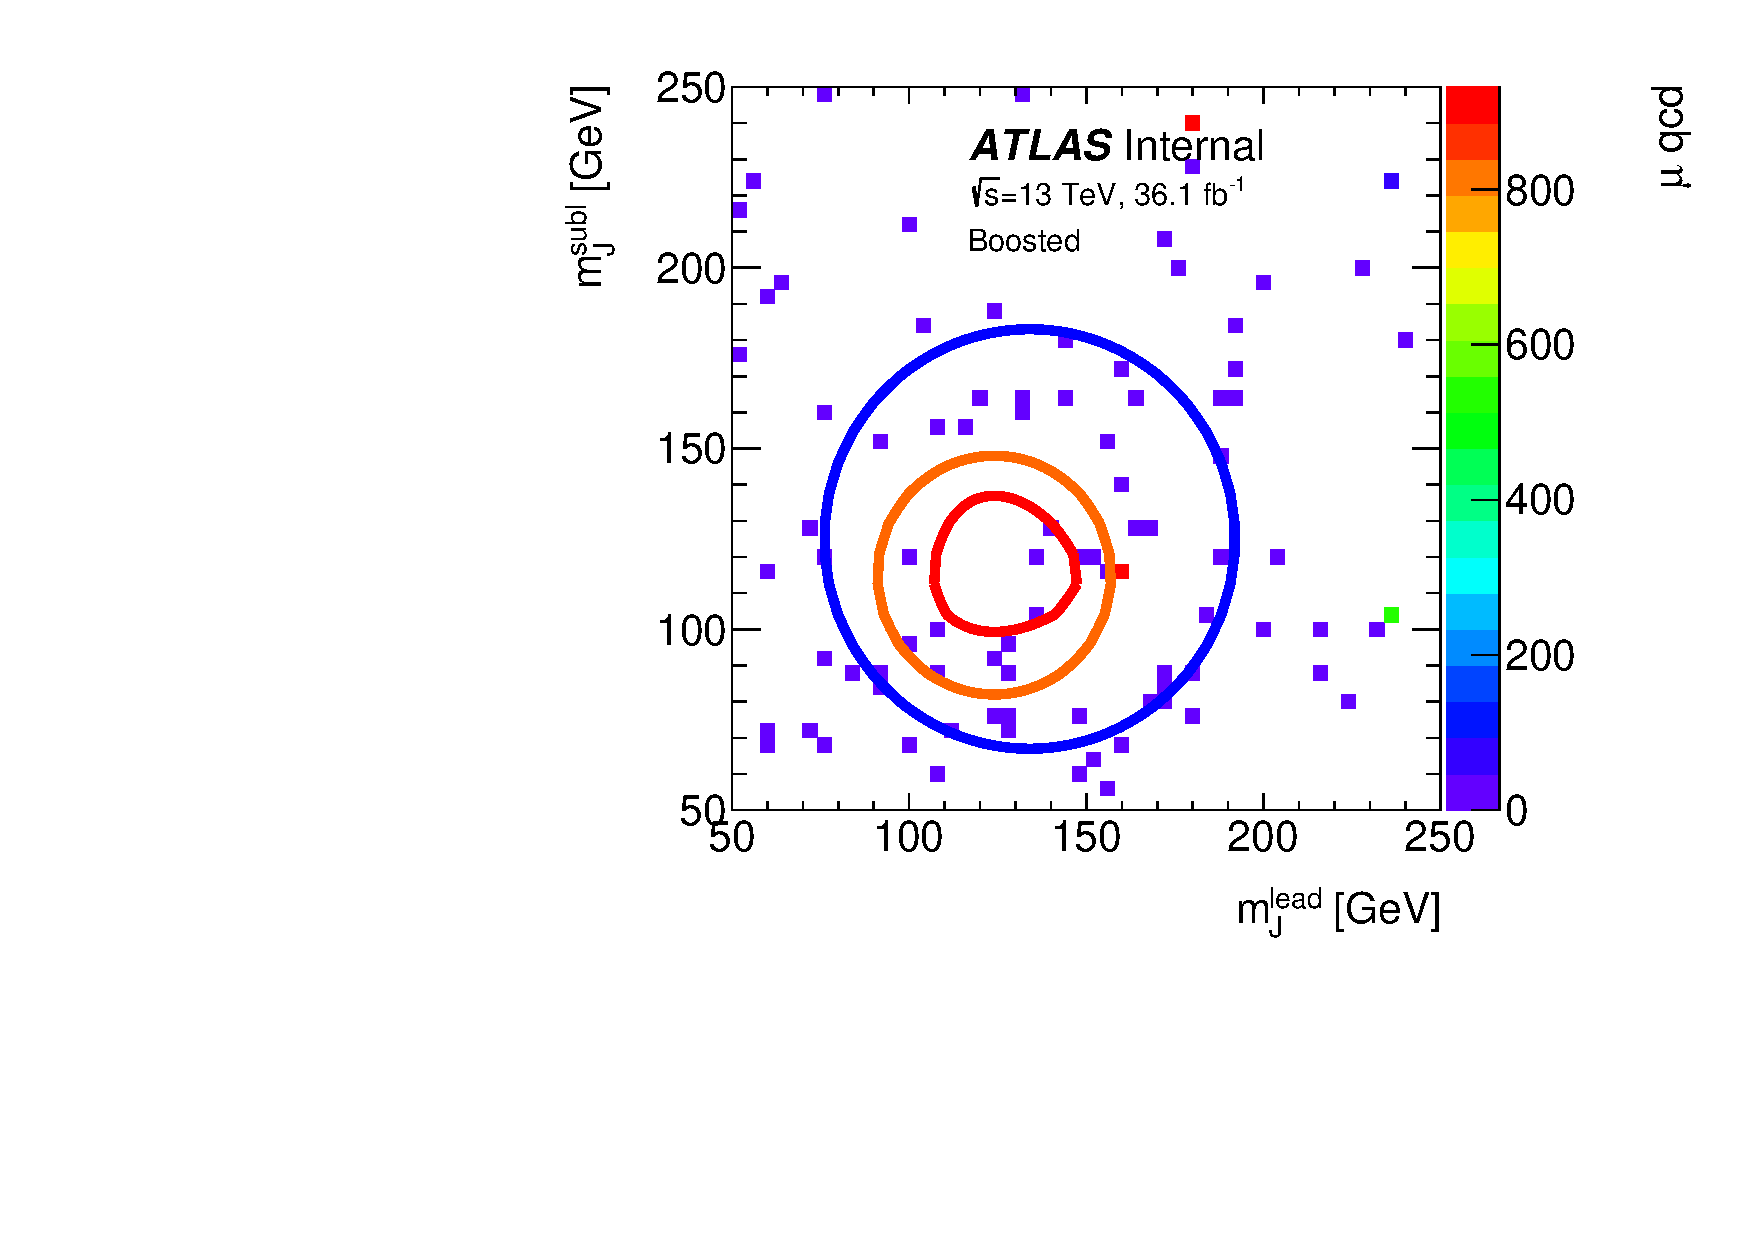
\includegraphics[width=\textwidth,angle=-90]{figures/boosted/AppendixMuqcdstudy/QCD_FourTag_Incl_mH0H1.pdf}
        \caption{\muqcd~ on the \mleadJ-\msublJ~ plane}
        \label{fig:app-muqcd-4b-2d-qcd}
    \end{subfigure}
    \quad \quad \quad \quad 
    \begin{subfigure}[b]{0.4\textwidth}
        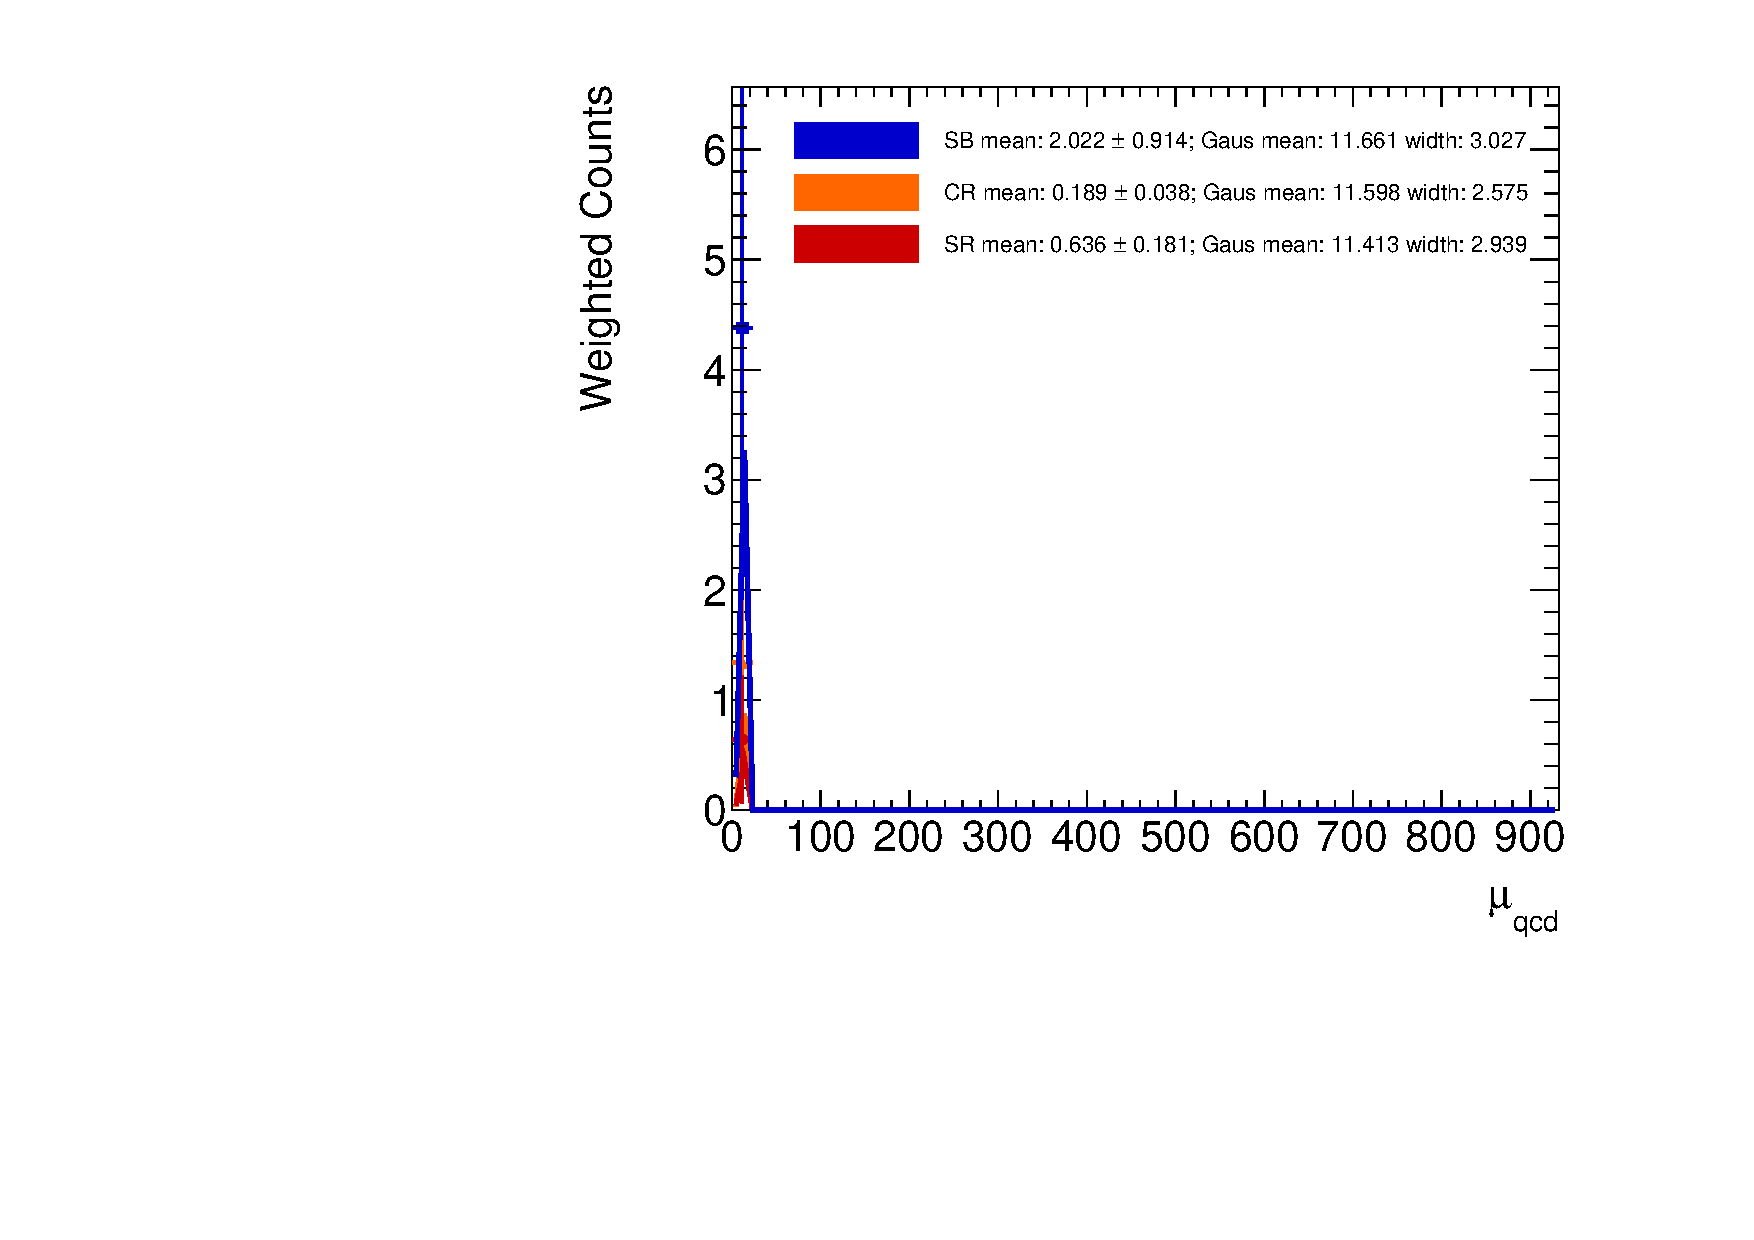
\includegraphics[width=\textwidth,angle=-90]{figures/boosted/AppendixMuqcdstudy/QCD_FourTag_Incl_mH0H1_pull.pdf}
        \caption{pulled \muqcd~ distribution in SB/CR/SR}
        \label{fig:app-muqcd-4b-pull-qcd}
    \end{subfigure}
\caption{$4b$ over $2b$ \muqcd~ values evaluated in dijet MC, with the $N_{event}$ weighted mean and the Gaussian fit mean listed.}
\label{fig:app-muqcd-4b-qcd}
\end{figure}